\documentclass[conference]{IEEEtran}
\IEEEoverridecommandlockouts
% The preceding line is only needed to identify funding in the first footnote. If that is unneeded, please comment it out.
\usepackage{cite}
\usepackage{amsmath,amssymb,amsfonts}
\usepackage{algorithmic}
\usepackage{graphicx}
\usepackage{listings}
\lstset{breaklines=true}
\usepackage{url}
\usepackage{hyperref}
\usepackage{dirtree}
\graphicspath{ {images/} }
\usepackage{textcomp}
\usepackage{xcolor}
\usepackage{todonotes}
\usepackage{subcaption}
\usepackage{placeins}
\usepackage{comment}
\usetikzlibrary{positioning}

\usepackage{tikz}
\usetikzlibrary{calc, patterns, patterns.meta, shapes.geometric, arrows.meta, positioning, fit, decorations.pathreplacing, trees, arrows, shapes.misc, angles, quotes}
%Go-kart command \gokart{"x"}{"y"}{"rot_in_deg"}
\def\gokart#1#2#3{
    \begin{scope}[shift={(#1,#2)}, rotate=#3]
        \begin{scope}[shift={(0,-0.85)}] %Offset so (x,y) is the front bumper
            %Front bumper
            \draw[very thick] (-0.7, 0.75) -- (-0.5, 0.85) -- (0.5, 0.85) -- (0.7, 0.75);
            %Body
            \draw[fill=gray!30] (-0.5,-0.75) rectangle (0.5,0.75);
            %Wheels
            \draw[fill=black, rounded corners=0.75] (-0.6,0.6) rectangle (-0.4, 0.3); % Front left
            \draw[fill=black, rounded corners=0.75] (0.6,0.6) rectangle (0.4, 0.3); % Front right
            \draw[fill=black, rounded corners=0.75] (-0.6,-0.6) rectangle (-0.4, -0.3); % Rear left
            \draw[fill=black, rounded corners=0.75] (0.6,-0.6) rectangle (0.4, -0.3); % Rear right
            %Rear bumper
            \draw[very thick] (-0.6, -0.75) -- (-0.5, -0.8) -- (0.5, -0.8) -- (0.6, -0.75);
        \end{scope}
    \end{scope}
}


\usepackage{siunitx} 
\sisetup{locale = US}
\DeclareSIUnit{\Bit}{Bit}
\DeclareSIUnit{\baud}{Baud}
\DeclareSIUnit{\frame}{f}

\def\BibTeX{{\rm B\kern-.05em{\sc i\kern-.025em b}\kern-.08em
    T\kern-.1667em\lower.7ex\hbox{E}\kern-.125emX}}


\pagestyle{plain}

\begin{document}

\title{Radar odometry using mmWave technology for SLAM applications.\\
{\large Leveraging mmWave Radar Sensor Technology for odometry estimation.}
}

\author{\IEEEauthorblockN{Luis Fernando Rodriguez Gutierrez}
\IEEEauthorblockA{\textit{Fachhochschule Dortmund} \\
\textit{M.Eng. Embedded Systems Engineering}\\
luis.rodriguez001@stud.fh-dortmund.de}

}


\maketitle


\begin{abstract}
The employment and integration of radar technologies for the implementation of odometry has recently emerged as a promissing alternative to traditional methods, which often rely on visual or LiDAR-based systems. 
Radar Technology is particularly advantageous due to its robustness in various environmental conditions, such as fog, rain, and dust, where other systems results may degrade.

This work focus in the estimation of the vehicle's ego-motion using a single mmWave radar sensor which is mounted in front of the vehicle. This to avoid extra hardware costs and complexity.

The proposed pipeline incorporates clustering techniques, point-to-point iterative closest point (ICP) optimization, and Doppler velocity augmentation to address the inherent challenges of sparse and noisy radar point clouds.
Notably, the point-to-point ICP approach is advantageous for radar-based odometry as it does not require an initial guess of the transformation, which is often difficult to obtain due to data sparsity and noise.
Furthermore, submap aggregation is employed to enhance registration stability across consecutive scans. Experimental evaluations demonstrate that the proposed framework enables consistent ego-motion estimation and highlights the potential of mmWave radar as a cost-efficient solution for autonomous navigation and digital twin construction in complex driving environments.

\end{abstract}

\begin{IEEEkeywords}
Radar Odometry, mmWave Radar, ICP, Doppler Velocity, Doppler Augmentation, Ego-Motion Estimation, Digital Twin
\end{IEEEkeywords}


\section{Introduction}
\label{sec:introduction}

Accurate and reliable ego-motion estimation is a fundamental requirement for mobile robotic systems and autonomous vehicle solutions.  
It is the basis for localization, mapping, and navigation, and errors in this stage directly affect the overall performance of autonomous systems.  

Traditionally, odometry has been estimated using a combination of wheel encoders, inertial measurement units (IMUs), and GPS.  
In more recent years, cameras and LiDAR have been widely used as they provide dense information about the environment, enabling precise feature extraction and recognition.  
However, these vision-based and LiDAR-based methods have significant drawbacks.  
Cameras are highly sensitive to illumination changes.  
LiDAR systems are costly, and their performance can degrade in adverse weather conditions such as fog, rain, or snow.  
Both methods also require high computational and memory resources.  
These limitations create the need for complementary sensing solutions that remain reliable under real-world conditions.  

Millimeter-wave (mmWave) radar has emerged as a strong candidate to address these issues.  
Radar is compact, cost-efficient, and inherently robust to poor lighting and weather.  
A key advantage of radar is its ability to directly measure Doppler velocity.  
Unlike cameras or LiDAR, which require frame-to-frame comparisons to estimate motion, radar provides direct measurements of radial velocity.  
This not only indicates how fast the vehicle is approaching or moving away from an object, but also makes it possible to separate static structures from moving objects and to detect relative motion trends.  
These Doppler-based measurements provide additional constraints for ego-motion estimation, making radar a unique and valuable sensing modality.  

Despite these advantages, radar data also presents challenges.  
The resulting point clouds are sparse and noisy, and they often include significant amounts of clutter.  
Radar also has lower angular resolution compared to LiDAR or cameras.  
These limitations make it difficult to directly apply traditional scan-matching techniques, which are usually designed for dense LiDAR point clouds.  
Previous work has shown that radar-only odometry and multimodal fusion can improve robustness, but challenges remain when dealing with sparsity, clutter, and the stability of scan registration.  

This work investigates the use of mmWave radar sensors mounted on a Ninebot Go-Kart \cite{ninebot_product_page} test platform.  
The system also integrates an IMU and an embedded processing unit.  
A visual overview of the setup, including sensor placement, is shown in Figure~\ref{fig:Ninebot_system}.  

\begin{figure}[!htbp]
    \centering
    \includegraphics[width=0.9\linewidth]{images/vehicleSystem.png}
    \caption{Ninebot test-vehicle system.}
    \label{fig:Ninebot_system}
\end{figure}

\newpage
The contributions of this work can be summarized as follows:  
\begin{enumerate}
    \item A radar ego-motion pipeline using mmWave sensors for displacement measurements and an IMU for rotation, minimizing hardware cost and system complexity.
    \item Integration of Doppler velocity and RANSAC filtering to improve the separation of static and dynamic objects.
    \item Submap aggregation to mitigate point cloud sparsity and improve alignment stability.
    \item Object tracking via clusters to identify and filter dynamic objects from the ego-motion estimation.
    \item Experimental validation using real-world data collected from a vehicle-mounted mmWave radar system.  
\end{enumerate}

\section{Objective and Sub-Tasks}
\label{sec:objective}
The main objective of this work is the development of a radar-based odometry system that estimates the vehicle ego-mmotion using mmWave radar sensors mounted at the fron of the vehicle setup in combination with an IMU for rotation compensation.
That motivation behind this approach is to explore radar as a cost-effective and robust alternative to the existing solutions based in vision or LiDAR-based odometry, particularly in conditions where those have the tendency to fail.
This builds on prior evidence that radar can support instantaneous ego-motion estimation through Doppler velocity cues \cite{EgoMotion_DopplerRadar}.

The system processes radar point cloud data enriched with range, angle, and most importantly Doppler velocity, to extract accurate motion estimates for ego-velocity or speed.
This enables the reconstruction of the vehicle’s trajectory and provides valuable input for SLAM applications.

\begin{figure}[!htbp]
    \centering
    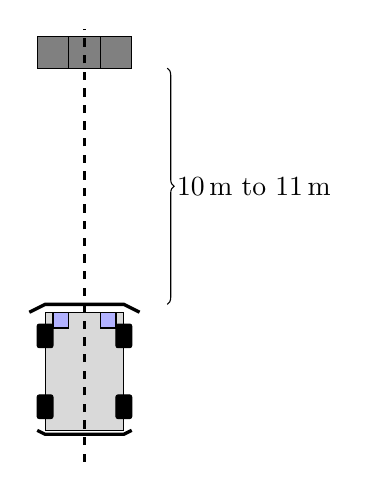
\begin{tikzpicture}
        \gokart{0}{0}{0}
    
        % Wall (three cubes)
        \draw[fill=gray] (-0.6,3) rectangle (-0.2,3.4);
        \draw[fill=gray] (-0.2,3) rectangle (0.2,3.4);
        \draw[fill=gray] (0.2,3) rectangle (0.6,3.4);
    
        % Dashed line from go-kart to wall (center axis)
        \draw[dashed, thick] (0,-2) -- (0,3.5);
    
        % Range brace annotation
        \draw [decorate, decoration = {brace, raise=10pt}] (0.7,3) -- (0.7, 0) node[pos=0.5,right=10pt,black]{\SIrange{10}{11}{\meter}};

        % Enlarged Radar sensor boxes
        \draw[fill=blue!30] (-0.4,-0.3) rectangle (-0.2,-0.1);

        \draw[fill=blue!30] (0.2,-0.3) rectangle (0.4,-0.1);
    \end{tikzpicture}
    \caption{Test scenario with dual front-mounted mmWave radar sensors.}
    \label{fig:test_scenario}
\end{figure}

The experimental setup is illustrated in Figure \ref{fig:test_scenario}, where two mmWave radar sensors are mounted at the front of a vehicle, providing overlapping fields of view to enhance environmental perception.
The dual-sensor configuration improves spatial coverage, reduces blind spots, and increases point density, resulting in more stable odometry processing compared to a single-sensor setup—an approach that aligns with multimodal methods for robust state estimation \cite{Multimodal_Offroad,HighSpeed_Estimation}.

By combining data from both sensors, including radial speed measurements derived from the Doppler effect, with the inertial measurement unit (IMU) for rotation compensation, the proposed system aims to ensure resilient odometry performance even under high-speed or degraded environmental conditions, where LiDAR-based odometry may fail \cite{HighSpeed_Estimation}.

Each radar perspective is processed independently and then merged into a single point cloud for further analysis.
This integration provides a more robust and reliable input to the odometry estimation pipeline, enabling the evaluation of radar-based odometry performance in realistic driving scenarios.

\subsection{Sub-Tasks}

The research objective, together with the constraints of using a dual-radar sensor, implied several practical sub-tasks:  
\begin{itemize}
    \item Designing a modular pipeline to acquire and decode synchronized radar data from both sensors.
    \item Investigating suitable sensor configurations to balance field of view, chirp bandwidth, update rate, and detection density.  
    \item Developing suitable mechanical mounts and selecting optimal sensor placement to ensure stability and maximize coverage.
    \item Applying RANSAC filtering on Doppler velocities to reject dynamic points and outliers.
    \item Implementing clustering methods to structure radar detections and isolate relevant features.  
    \item Optimizing the raw radar point cloud using additional information provided by the sensor itself (e.g., SNR, RCS, or range validity) to improve reliability before odometry processing.  
    \item Integrating Doppler velocity information into the odometry estimation process.   
    \item Employing submap aggregation to mitigate sparsity and improve stability. 
    \item Performing ICP alignment between submaps aggregated from both sensors to mitigate sparsity and noise. 
    \item Evaluating the influence of the dual-sensor arrangement on odometry accuracy and robustness. 
    \item Validating the complete system on real-world driving scenarios. 
\end{itemize}

As each sub-task builds upon the results of the previous one, the work followed an iterative and modular development approach, enabling gradual integration and continuous evaluation of the proposed system.  
The following sections detail the implementation and evaluation of each sub-task, culminating in a comprehensive radar-based odometry solution.
\section{IWR6843 Radar Interface and Configuration}
\label{sec:IWR6843 Radar Interface and Configuration}
The IWR6843AOPEVM development board from Texas Instruments features the IWR6843AOP, a high performance 4D mmWave FMCW sensor with Antenna On Package (AOP) design.
Although IWR6843AOP is intended for industrial applications and its complementary chip, AWR6843AOP, for automotive applications, IWR6843AOP was used in this project because it is available in the form of this development board and the two chips are identical in terms of their functionalities, only differing in compliance with automotive  industry \cite{iwr_awr_diff}.
Its small physical size, due to its AOP design, makes it an optimal choice for the desired mounting position, the go-kart's steering column.
\begin{figure}[!htbp]
    \centering
    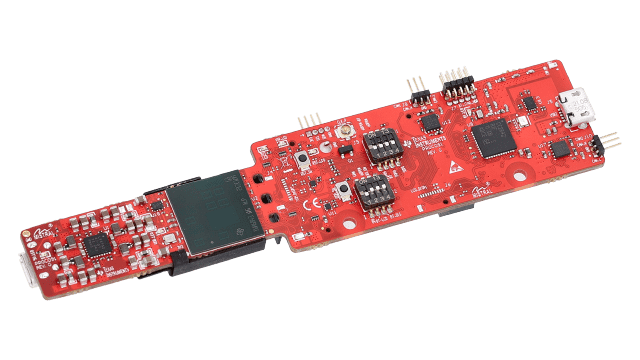
\includegraphics[width=0.7\linewidth]{images/iwr6843aopevm-angled.png}
    \caption{IWR6843AOP sensor\\
    \textit{Source: Texas Instruments, available at \url{https://www.ti.com/ds_dgm/images/fbd_swrs219f.gif}}}
    \label{fig:IWR6843AOP sensor}
\end{figure}
\par
The IWR6843AOP radar sensor operates within the frequency range of \SIrange{60}{64}{\giga\hertz} and integrates 4 receive (RX) and 3 transmit (TX) antennas, radio frequency (RF) front-end stages, analog signal processing, and digital signal processing (DSP).
It offers a wide range of communication interfaces including SPI, I2C, CAN-FD, UART and LVDS for raw data access and an Arm Cortex-R4F microcontroller for user-applications \cite{dev_board_page}.

\begin{figure}[!htbp]
    \centering
    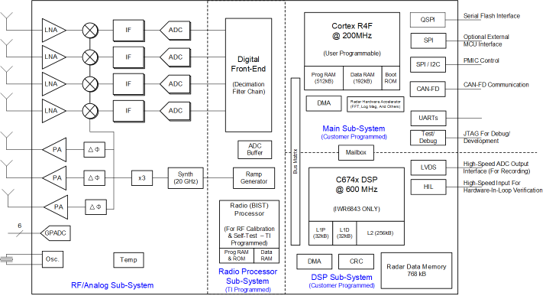
\includegraphics[width=1.0\linewidth]{images/blockdiagram.png}
    \caption{IWR6843AOP internal block diagram.\\
    \textit{Source: Texas Instruments, available at \url{https://www.ti.com/ds_dgm/images/fbd_swrs219f.gif}}}
    \label{fig:IWR6843AOP_internal}
\end{figure}

\FloatBarrier\noindent
Texas Instruments offers various demo applications for the development board that utilize the internal microcontroller for showcasing the radar sensor's capabilities in different specialized scenarios.
It was found out that most of them only use the radar sensor itself only for obtaining a point cloud, which points include spatial information in form of $x,y,z$ coordinates and a radial speed information (the prior mentioned four dimensions of the sensor).
Application-specific processing of the point cloud itself is executed on an external computation device.
\par
The main demo application ("mmWave SDK demo") allows a versatile customization of the radar sensor's operating parameters and its discrimination capabilities while outputting the point cloud via its UART interface, accessible via the on-board USB to UART converter.
Although the demo seems to be intended to be used only for demonstration purposes, many projects based on Texas Instruments' mmWave radar sensors utilize it, because it poses a generic solution for obtaining (close to) real-time point cloud data from the sensor without prior development of a custom user-application for the radar sensor's internal microcontroller.
This setup was therefore chosen for supplying the emergency braking system with data.

\subsection{Utilizing the mmWave SDK demo}
The "mmWave SDK demo" was developed by Texas Instruments for showcasing the abilities of their mmWave radar sensors.
It consists of the radar sensor itself, supplying close to real-time point cloud data and an online tool for visualization of the raw output data and for the creation of a sequence of commands used for configuration of the radar sensor's operating parameters and output \cite{mmwave_demo_doc}.
Due to the demo's simple structure and the radar sensor's generic output, the online application can be replaced by a custom application replicating the online tool's behavior for making use of the data.
\par
In the demo application, the radar sensor opens two UART connections.
One connection is bidirectional at a lower speed of \SI{115200}{\baud} which is used to configure the radar sensor by sending the previously mentioned sequence of commands. 
The second connection is unidirectional, from the radar sensor to the receiver, at a higher speed of \SI{921600}{\baud} and is used for outputting a constant data stream after the radar sensor received its configuration and a start command.
As the data packets are encoded in a proprietary format and therefore need to be parsed prior to further processing, a custom software module was written in C++ and later ported to Python.
The module handles the radar sensor's setup by sending a configuration file containing the sequence of initialization commands and the cyclic parsing of the encoded data packets.
The sequence of commands was generated with Texas Instruments' online tool, as it provided graphical feedback while making the necessary compromises involved in setting up the radar sensor's operating parameters.

\subsection{Sensor Data Output Format}
As the data packets, containing the individual frames, are encoded in a proprietary format, they need to be parsed to allow for further processing.
Each frame starts with a frame header and contains a number of TLVs (Type, Length, Value) in which the actual payload data is stored\cite{mmwave_demo_doc}.
\begin{figure}[!htbp]
    \centering
    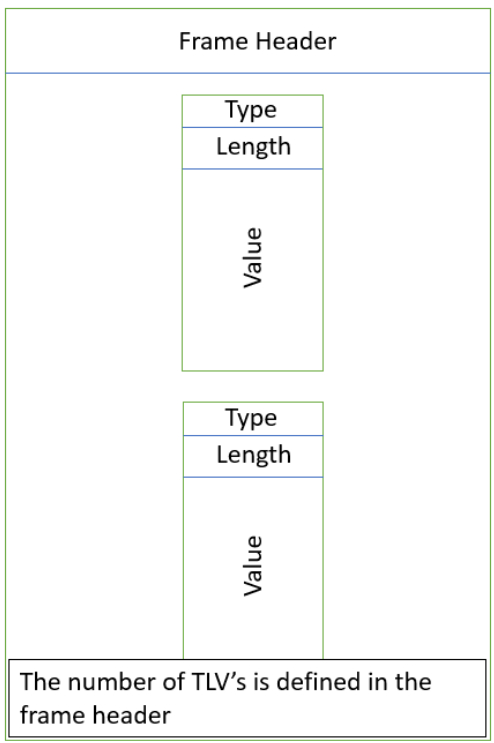
\includegraphics[width=0.4\linewidth]{images/UARTFrame.png}
    \caption{Frame structure. From \cite{mmwave_demo_output}.\\
    \textit{Source: Texas Instruments, available at \url{https://dev.ti.com/tirex/content/radar_toolbox_2_20_00_05/docs/software_guides/Understanding_UART_Data_Output_Format.html}}}
    \label{fig:UART data output format}
\end{figure}
\FloatBarrier\noindent
The frame's header has a total length of \SI{40}{\byte} and starts with a fixed magic word that denotes the start of each frame.
It also provides several other information in addition to the total packet length in bytes which is used to find the frame's end:
\begin{itemize}
    \item Magic Word: This value indicates the start of a new header, meaning that it can be used as a starting point for processing each frame.
    \item Total Packet Length: Total number of bytes in the frame (including the header) which can be used to calculate the frame's end.
    \item Platform: Indicates the device type and can be used for validating the radar sensor type. In the case of the device used for this project (IWR6843AOP) the expected value is "$0xA6843$".
    \item Number of TLVs: Total number of TLV's that exist in that specific frame.
\end{itemize}
\begin{figure}[!htbp]
    \centering
    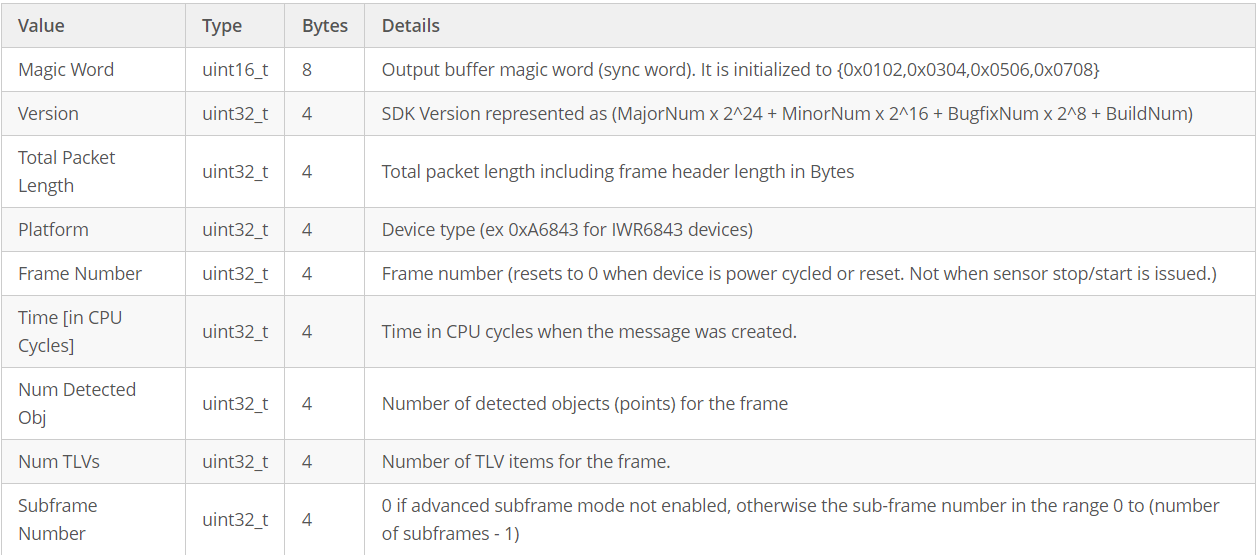
\includegraphics[width=1.0\linewidth]{images/FrameFormatHeader.png}
    \caption{Frame header format. From \cite{mmwave_demo_output}.\\
    \textit{Source: Texas Instruments, available at \url{https://dev.ti.com/tirex/content/radar_toolbox_2_20_00_05/docs/software_guides/Understanding_UART_Data_Output_Format.html}}}
    \label{fig:Frame header format}
\end{figure}
\FloatBarrier\noindent
The frame contains one or more TLVs after its header.
Each TLV has a header itself in which it specifies its length and which type of data (point cloud, doppler heatmaps, statistics, ...) is contained inside.
Each TLV type needs to be decoded differently, as it represents a different type of data.
\begin{figure}[!htbp]
    \centering
    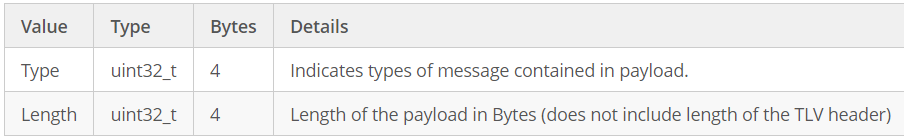
\includegraphics[width=0.95\linewidth]{images/TLVHeader.png}
    \caption{TLV header format. From \cite{mmwave_demo_output}.\\
    \textit{Source: Texas Instruments, available at \url{https://dev.ti.com/tirex/content/radar_toolbox_2_20_00_05/docs/software_guides/Understanding_UART_Data_Output_Format.html}}}
    \label{fig:TLV header format}
\end{figure}
\FloatBarrier

\subsection{Sensor-Tuning}
As some operating parameters influence each other, their selection must be done carefully while observing the influence of the trade-offs involved.
This could be referred to as "sensor tuning" and is a critical step because it directly impacts the system's accuracy and performance.

The following operating parameters can be tuned:
\begin{itemize}
    \item Frame rate
    \item Range resolution
    \item Maximum unambigious range
    \item Maximum radial velocity
    \item Radial velocity resolution
\end{itemize}

Tuning these operating parameters introduces trade-offs by influencing each other in the following ways:
\begin{table}[h]
    \centering
    \resizebox{\columnwidth}{!}{
    \begin{tabular}{|l|l|p{3.5cm}|p{3.5cm}|p{3.5cm}|}
        \hline
        \textbf{Tuning Parameter} & \textbf{Effect on Performance} & \textbf{Related HW Block} & \textbf{Trade-Off} \\
        \hline
        Frame Rate & Higher FPS = faster updates but more processing load & C674x DSP, Radar Data Memory & Higher FPS reduces maximum range \\
        \hline
        Range Resolution & Higher resolution = better object separation & ADC, 1D FFT (Range FFT) & Higher resolution reduces max range \\
        \hline
        Maximum Range & Determines farthest detectable object & RF Front-End, PA, LNA, ADC & Higher range lowers resolution \\
        \hline
        Radial Velocity Resolution & Improves speed accuracy & DSP, 2D FFT (Doppler FFT) & Higher resolution requires more chirps \\
        \hline
        Maximum Radial Velocity & Detects fast-moving objects & Chirp rate, TX Antennas, 2D FFT & Higher max velocity reduces resolution \\
        \hline
    \end{tabular}
    }
    \caption{Radar System Tuning Parameters and Trade-offs}
    \label{tab:mmWave_Sensor_Parameters}
\end{table}
The resulting overall accuracy of the velocity and distance measurements is again dependent on these operating parameters:
\begin{itemize}
\item \textbf{Radial velocity accuracy:} A fine balance between velocity resolution and frame rate must be maintained to ensure precise Doppler shift measurements. Lower resolution results in rounded velocity values, while an excessively high frame rate may introduce computational bottlenecks.
\item \textbf{Distance accuracy:} Optimizing range resolution and maximum range ensures that detected objects are positioned accurately within the environment. Increasing range often sacrifices resolution, leading to potential inaccuracies in close-range detections.
\item \textbf{Signal processing considerations:} The FFT calculation parameters directly affect both range and Doppler calculations, influencing the ability to distinguish between objects and detect small velocity variations.
\end{itemize}

This shows that finding exact values for the operation parameters by adjusting them while carefully watching their influences is crucial and heavily dependent on the particular application.
The test scenario required a frame rate of approximately 30Hz to balance responsiveness and computational load, together with sufficient range and velocity coverage to capture typical vehicle dynamics.

The resulting configuration yielded the following operating parameters:
\begin{itemize}
\item Frame rate: \SI{30}{\frame\per\second}
\item Range resolution: \SI{0.047}{\meter}
\item Maximum unambiguous range: \SI{9.78}{\meter}
\item Maximum radial velocity: \SI{8.01}{\meter\per\second}
\item Radial velocity resolution: \SI{0.51}{\meter\per\second}
\end{itemize}

Tuning and choosing the sensor's parameters carefully is extremely important as it defines the accuracy of 
therefore influences the reliability of the entire radar system.
Fine-tuning these settings ensures that the sensor operates optimally, enabling more precise self-speed estimation and overall system performance.
The accuracy of radial speed estimation and distance measurements depends directly on the tuning of these parameters. A poorly configured sensor can result in erroneous velocity estimations, unreliable object detection, or excessive noise in Doppler measurements. 
An example of the influence of the selection of the correct parameters on the output point cloud of the radar sensor can be found in Fig.~\ref{fig:IWR6843AOP Calibration example2 for the sensor}.

\begin{figure}[!htbp]
    \centering
    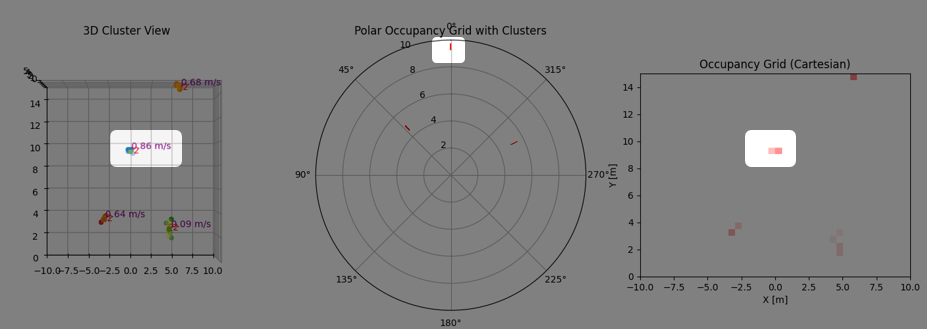
\includegraphics[width=1.0\linewidth]{images/calib_ex.png}
    \caption{Output of the IWR6843AOP prior sensor tuning.}
    \label{fig:IWR6843AOP Calibration example for the sensor}
\end{figure}

\begin{figure}[!htbp]
    \centering
    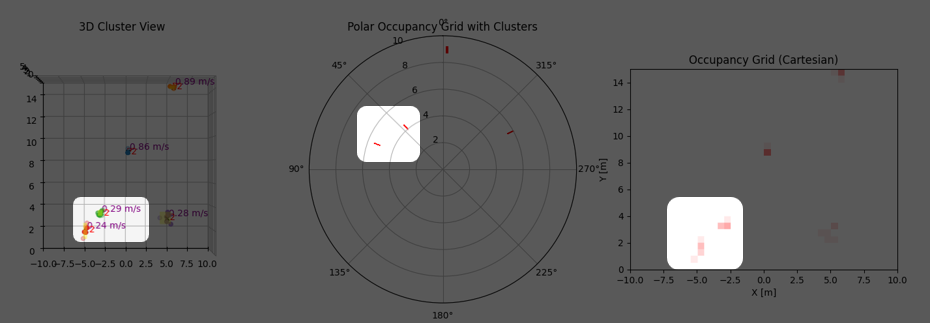
\includegraphics[width=1.0\linewidth]{images/calib_ex2.png}
    \caption{Output of the IWR6843AOP after sensor tuning.}
    \label{fig:IWR6843AOP Calibration example2 for the sensor}
\end{figure}

\subsection{Dual Sensor-Tuning} 
In addition to the individual calibration of each radar, further adjustments were required to enable a dual-sensor configuration with overlapping fields of view. 
The sensors were physically rotated around the $Z$-axis to widen the horizontal coverage and tilted by $15^\circ$ around the $X$-axis to prevent ground reflections and reduce clutter in the point clouds. 

\subsubsection{Chirp Calibration with Frequency Shift} 
Although both sensors operated under the same high-level parameters, their chirps had to be tuned to avoid mutual interference and ghost detections. 
To achieve this, each radar was configured to occupy only 2\,GHz of the available 4\,GHz bandwidth, introducing a frequency shift between the sensors. 
The resulting chirp design was derived using the Texas Instruments \textit{mmWave Sensing Estimator} tool \cite{understanding_uart}, which provides interactive validation of scene-dependent parameters, chirp design, and power consumption estimates. 
This configuration allowed the sensors to operate simultaneously without cross-talk while maintaining sufficient range resolution and velocity accuracy. 

\subsubsection{Geometric Transformations} 
To merge both radar outputs into a consistent reference frame, rigid-body transformations were applied to compensate for rotation, tilt, and translation offsets between the sensors. 
Each radar detections were first processed in its local coordinate frame and then transformed into the vehicle-centric frame before fusion into a single point cloud. 

Figures~\ref{fig:dualSensorCalib_rawComparison}--\ref{fig:dualSensorCalib_RANSACComparison} illustrate the effect of this calibration process at different processing stages: 
\begin{itemize} 
    \item \textbf{Raw point clouds:} Before calibration (Fig.~\ref{fig:dualSensorCalib_rawComparison}a), the detections from each sensor appear misaligned, producing duplicated landmarks. After applying the transformations (Fig.~\ref{fig:dualSensorCalib_rawComparison}b), both perspectives are fused into a coherent scene. 
    \item \textbf{Clustered view:} When clustering is applied, the uncalibrated data (Fig.~\ref{fig:dualSensorCalib_clusterComparison}a) shows inconsistent cluster centers, while the calibrated version (Fig.~\ref{fig:dualSensorCalib_clusterComparison}b) produces compact and aligned clusters. 
    \item \textbf{RANSAC Doppler fitting:} Similarly, Doppler–azimuth consistency improves after calibration. Uncalibrated detections (Fig.~\ref{fig:dualSensorCalib_RANSACComparison}a) yield noisier distributions, while the calibrated outputs (Fig.~\ref{fig:dualSensorCalib_RANSACComparison}b) produce smoother fits with fewer outliers. 
\end{itemize} 

The transformed data thus provides a coherent and stable input for the odometry estimation pipeline, ensuring that static landmarks are consistently aligned across both sensors.  

\begin{figure}[ht]
    \centering
    \begin{subfigure}[b]{0.45\textwidth}
        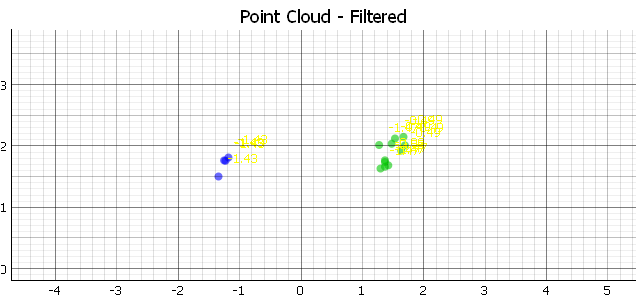
\includegraphics[width=\textwidth]{images/dualSensorCalib_2mts.png}
        \caption{Raw point cloud before calibration}
    \end{subfigure}
    \hfill
    \begin{subfigure}[b]{0.45\textwidth}
        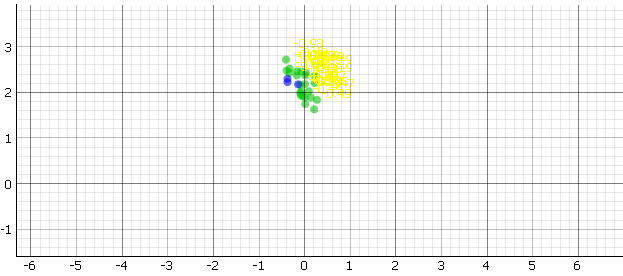
\includegraphics[width=\textwidth]{images/AFTERdualSensorCalib_2mts.png}
        \caption{Raw point cloud after calibration}
    \end{subfigure}
    \caption{Dual-sensor raw detections before and after applying geometric transformations.}
    \label{fig:dualSensorCalib_rawComparison}
\end{figure}

\begin{figure}[ht]
    \centering
    \begin{subfigure}[b]{0.3\textwidth}
        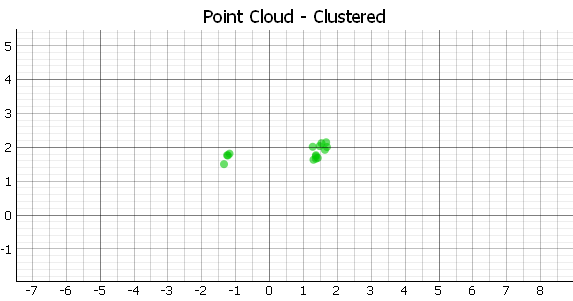
\includegraphics[width=\textwidth]{images/dualSensorCalibCluster_2mts.png}
        \caption{Clustered detections before calibration}
    \end{subfigure}
    \hfill
    \begin{subfigure}[b]{0.3\textwidth}
        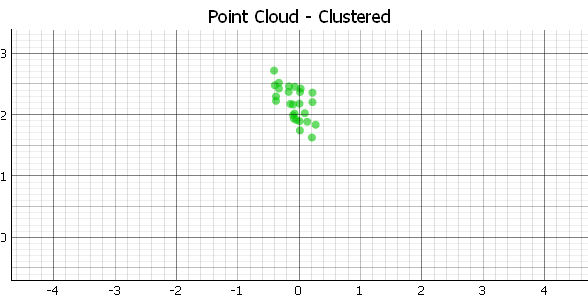
\includegraphics[width=\textwidth]{images/AFTERdualSensorCalibCluster_2mts.png}
        \caption{Clustered detections after calibration}
    \end{subfigure}
    \caption{Effect of calibration on cluster alignment across sensors.}
    \label{fig:dualSensorCalib_clusterComparison}
\end{figure}

\begin{figure}[ht]
    \centering
    \begin{subfigure}[b]{0.3\textwidth}
        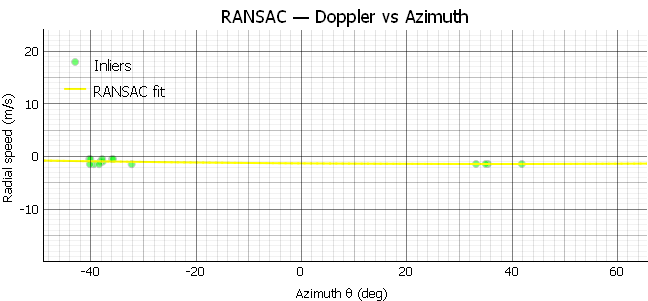
\includegraphics[width=\textwidth]{images/dualSensorCalibRANSAC_2mts.png}
        \caption{RANSAC Doppler fitting before calibration}
    \end{subfigure}
    \hfill
    \begin{subfigure}[b]{0.3\textwidth}
        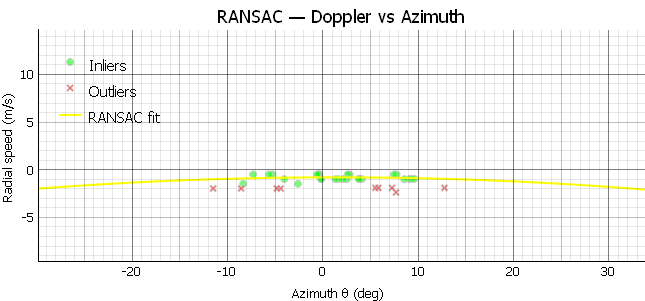
\includegraphics[width=\textwidth]{images/AFTERdualSensorCalibRANSAC_2mts.png}
        \caption{RANSAC Doppler fitting after calibration}
    \end{subfigure}
    \caption{Improvement in Doppler-azimuth consistency after calibration.}
    \label{fig:dualSensorCalib_RANSACComparison}
\end{figure}

\FloatBarrier
\section{CHIRP Sequence Configuration}

\label{sec:chirp-theory}

To enable effective ego-motion estimation, the radar must be configured with a suitable chirp profile that balances range and velocity resolution.
This is achieved through the configuration of Frequency-Modulated Continuous Wave (FMCW) chirps, which define how the radar sweeps frequencies over time to capture environmental information.

In millimeter-wave FMCW radar systems such as the IWR6843, a chirp refers to a signal whose frequency increases (or decreases) linearly over a defined bandwidth $B$ during a fixed duration $T_c$.
When this signal reflects off a target and returns to the radar, the delay between transmitted and received signals encodes range information.
The Doppler shift between multiple received chirps in a frame encodes relative velocity.  
As seen in Figure~\ref{fig:radarWavePropagation}, the reflected wave varies in phase and frequency depending on object motion.


\begin{figure}[!htbp]
    \centering
    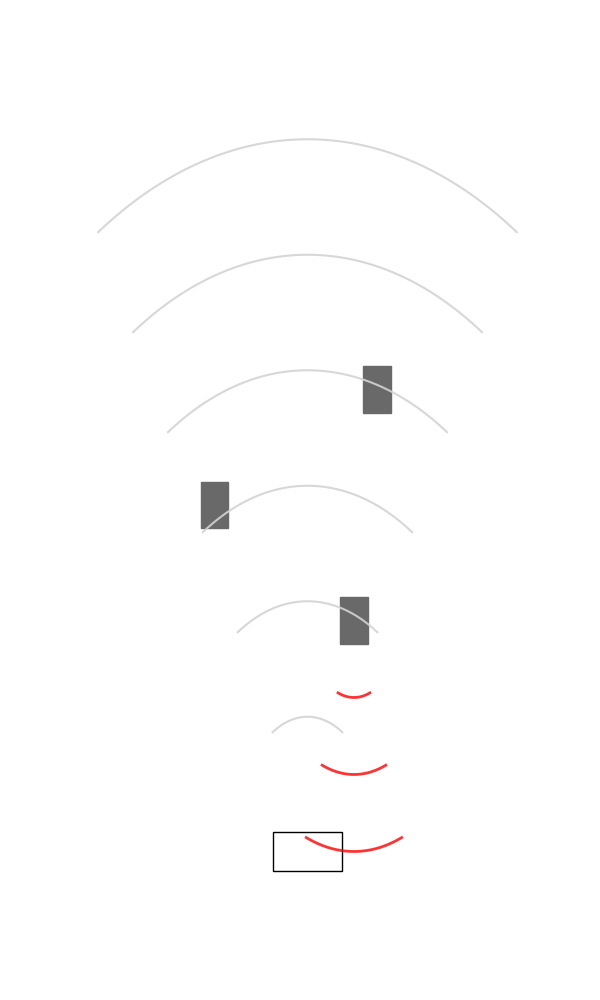
\includegraphics[width=0.5\linewidth]{images/radarWave.png}
    \caption{Radar 60-64GHz radio wave reflection.}
    \label{fig:radarWavePropagation}
\end{figure}

Each chirp is defined by the following core parameters:
\begin{itemize}
    \item Start frequency $f_0$
    \item Frequency slope $S$
    \item Chirp duration $T_c$
    \item Idle time between chirps $T_{idle}$
    \item Sampling rate $f_s$
    \item Bandwidth $B = S \cdot T_c$
\end{itemize}

\hfill

From these parameters, the radar sensing capabilities are derived as follows:

\begin{itemize}
    \item \textbf{Range resolution:} 
    \[
        \Delta R = \frac{c}{2B}
    \]
    where $c$ is the speed of light and $B$ is the chirp bandwidth.

    \item \textbf{Maximum unambiguous range:} 
    \[
        R_{max} = \frac{c f_s}{2S}
    \]
    where $f_s$ is the ADC sampling rate and $S$ is the frequency slope.

    \item \textbf{Velocity resolution:} 
    \[
        \Delta v = \frac{\lambda}{2 N_c T_c}
    \]
    where $\lambda$ is the wavelength, $N_c$ is the number of chirps per frame, and $T_c$ is the chirp duration.

    \item \textbf{Maximum unambiguous velocity:} 
    \[
        v_{max} = \frac{\lambda}{4 T_c}
    \]
    assuming uniform chirp spacing.
\end{itemize}

These equations clearly show that both range and velocity resolution depend directly on the chirp design.

\vspace{1em}
\newpage

\subsection{Chirp Design Strategies and Trade-offs}
\label{sec:chirp-strategies}

Radar applications differ in their emphasis on range vs velocity accuracy.
Odometry requires both.
We now examine key chirp configuration strategies and discuss their trade-offs.
\vspace{1em}

\subsubsection*{(1) Full-Bandwidth Chirp (Single 4~GHz Sweep)}

A single chirp sweeping across the entire 4~GHz available bandwidth provides the finest possible range resolution.
This is ideal for tasks requiring precise spatial localization of static objects.

\textbf{Trade-offs:}
\begin{itemize}
    \item \textbf{Pros:} Excellent range resolution ($\Delta R$ minimized).
    \item \textbf{Cons:} High ADC sampling rates required. Limits maximum measurable range ($R_{max}$). Increases noise sensitivity. Not ideal for multi-radar systems due to potential mutual interference.
\end{itemize}

\begin{figure}[!htbp]
    \centering
    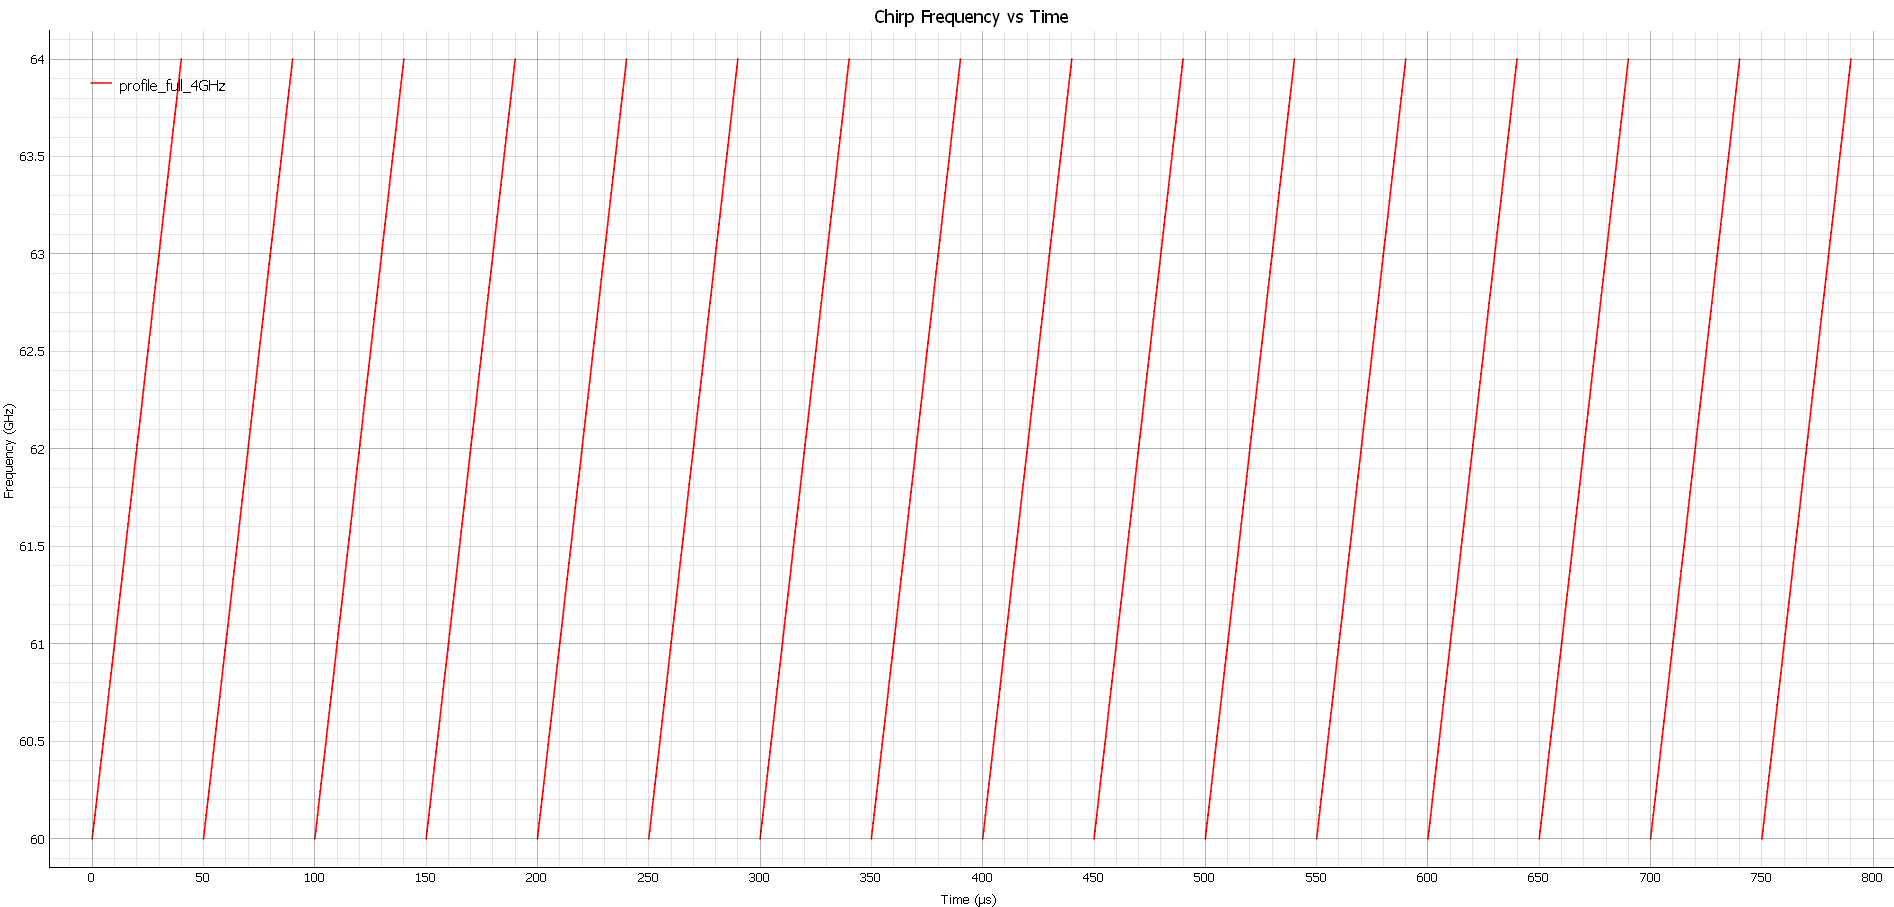
\includegraphics[width=1.0\linewidth]{images/profile_full_4GHz.png}
    \caption{Single 4~GHz chirp.}
    \label{fig:profile4GHz}
\end{figure}

{\small
\textit{Conclusion:} Best for high-resolution mapping in single-device systems.
May suffer in multi-radar setups due to wide spectral overlap.
}

\vspace{1em}

\subsubsection*{(2) Divided-Band Chirps (Multiple Shorter Sweeps)}

An alternative is to split the full 4~GHz bandwidth into multiple chirps with reduced individual sweep widths (e.g., 2~GHz).
Each chirp provides moderate resolution.

\textbf{Trade-offs:}
\begin{itemize}
    \item \textbf{Pros:} Reduced ADC load. Allows frequency diversity across chirps.
    \item \textbf{Cons:} Each individual chirp has worse $\Delta R$ than full sweep. However, averaging multiple bands improves robustness.
\end{itemize}

\begin{figure}[!htbp]
    \centering
    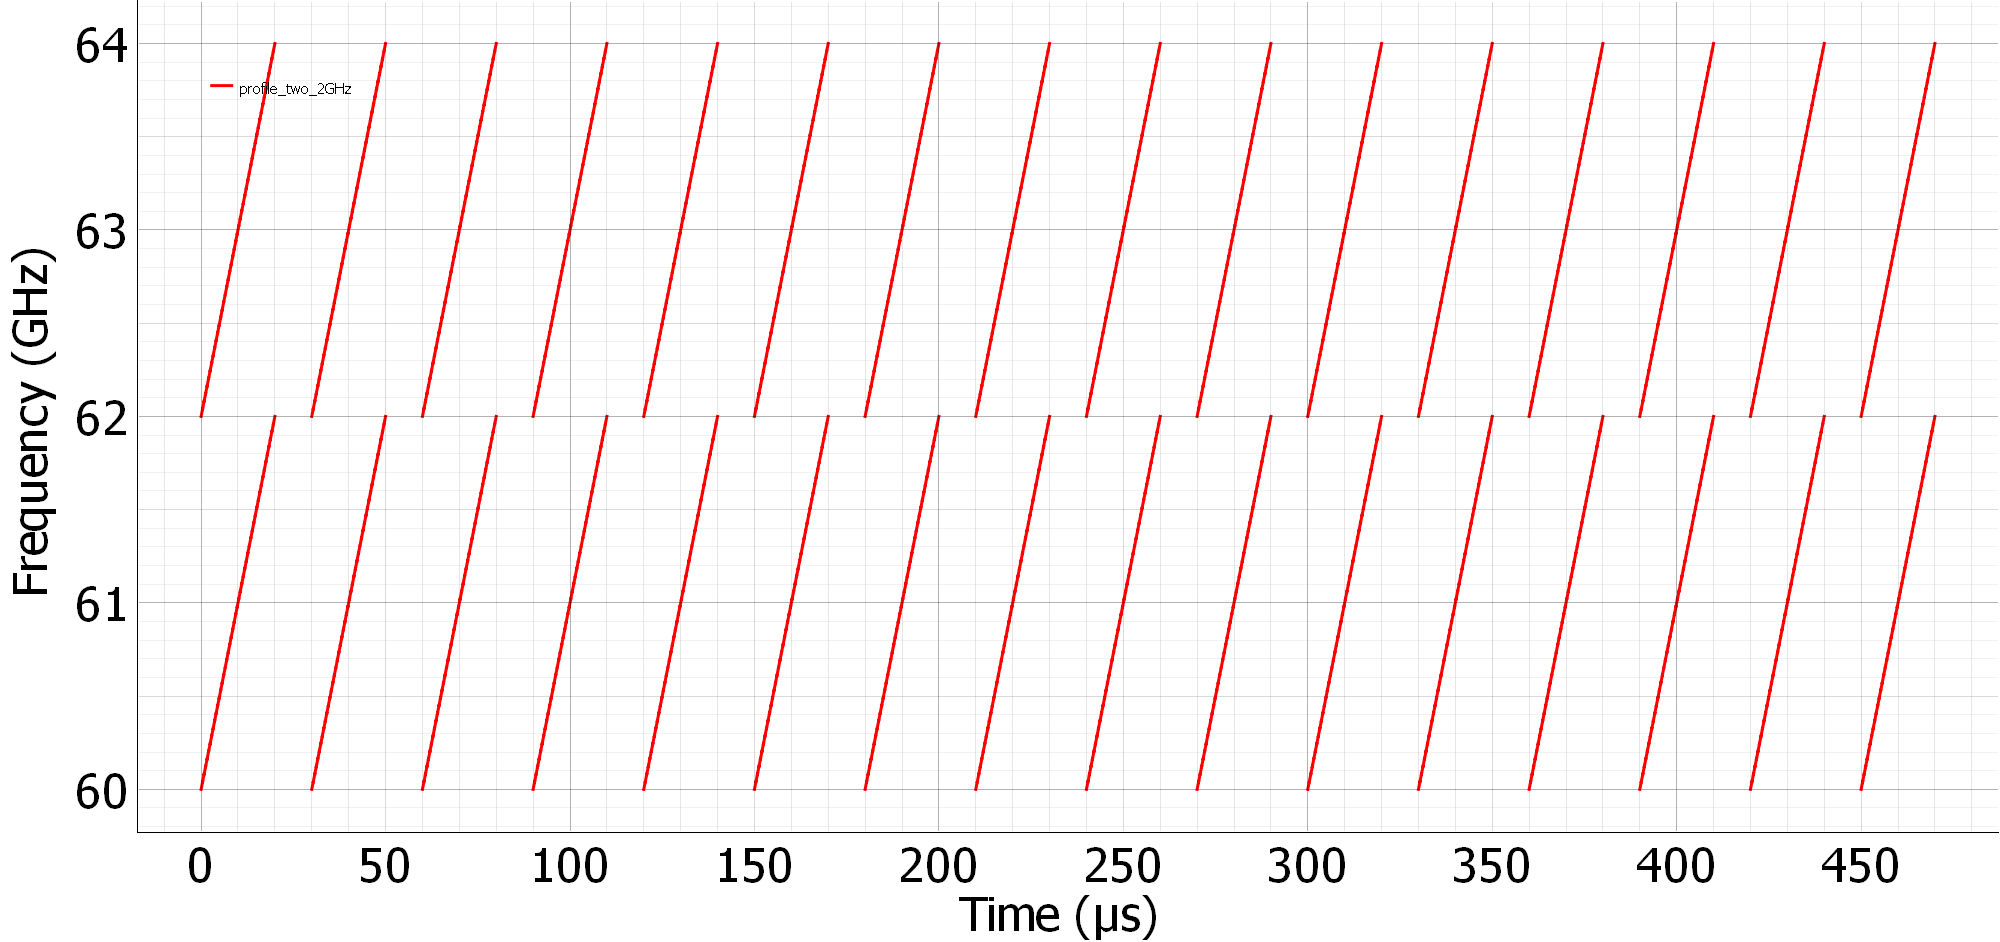
\includegraphics[width=1.0\linewidth]{images/profile_two_2GHz.png}
    \caption{Two 2~GHz chirps in the same frame.}
    \label{fig:profile2GHz}
\end{figure}

{\small
\textit{Conclusion:} Balanced design.
Useful in scenarios requiring robustness against channel noise or radar interference.
Also reduces overlap when multiple radars are active.
}

\vspace{1em}

\subsubsection*{(3) Mixed Chirp Strategy (Full-Band + Narrow-Band Chirps)}

Combining different chirp types in a single frame can provide both high range and velocity resolution.
For example, use one full-band chirp for precise range, followed by multiple narrow-band chirps for velocity estimation.

\textbf{Trade-offs:}
\begin{itemize}
    \item \textbf{Pros:} Leverages benefits of both strategies. Improves multi-parameter resolution without overwhelming hardware.
    \item \textbf{Cons:} Increases configuration complexity. Requires advanced processing and careful interleaving.
\end{itemize}

\begin{figure}[!htbp]
    \centering
    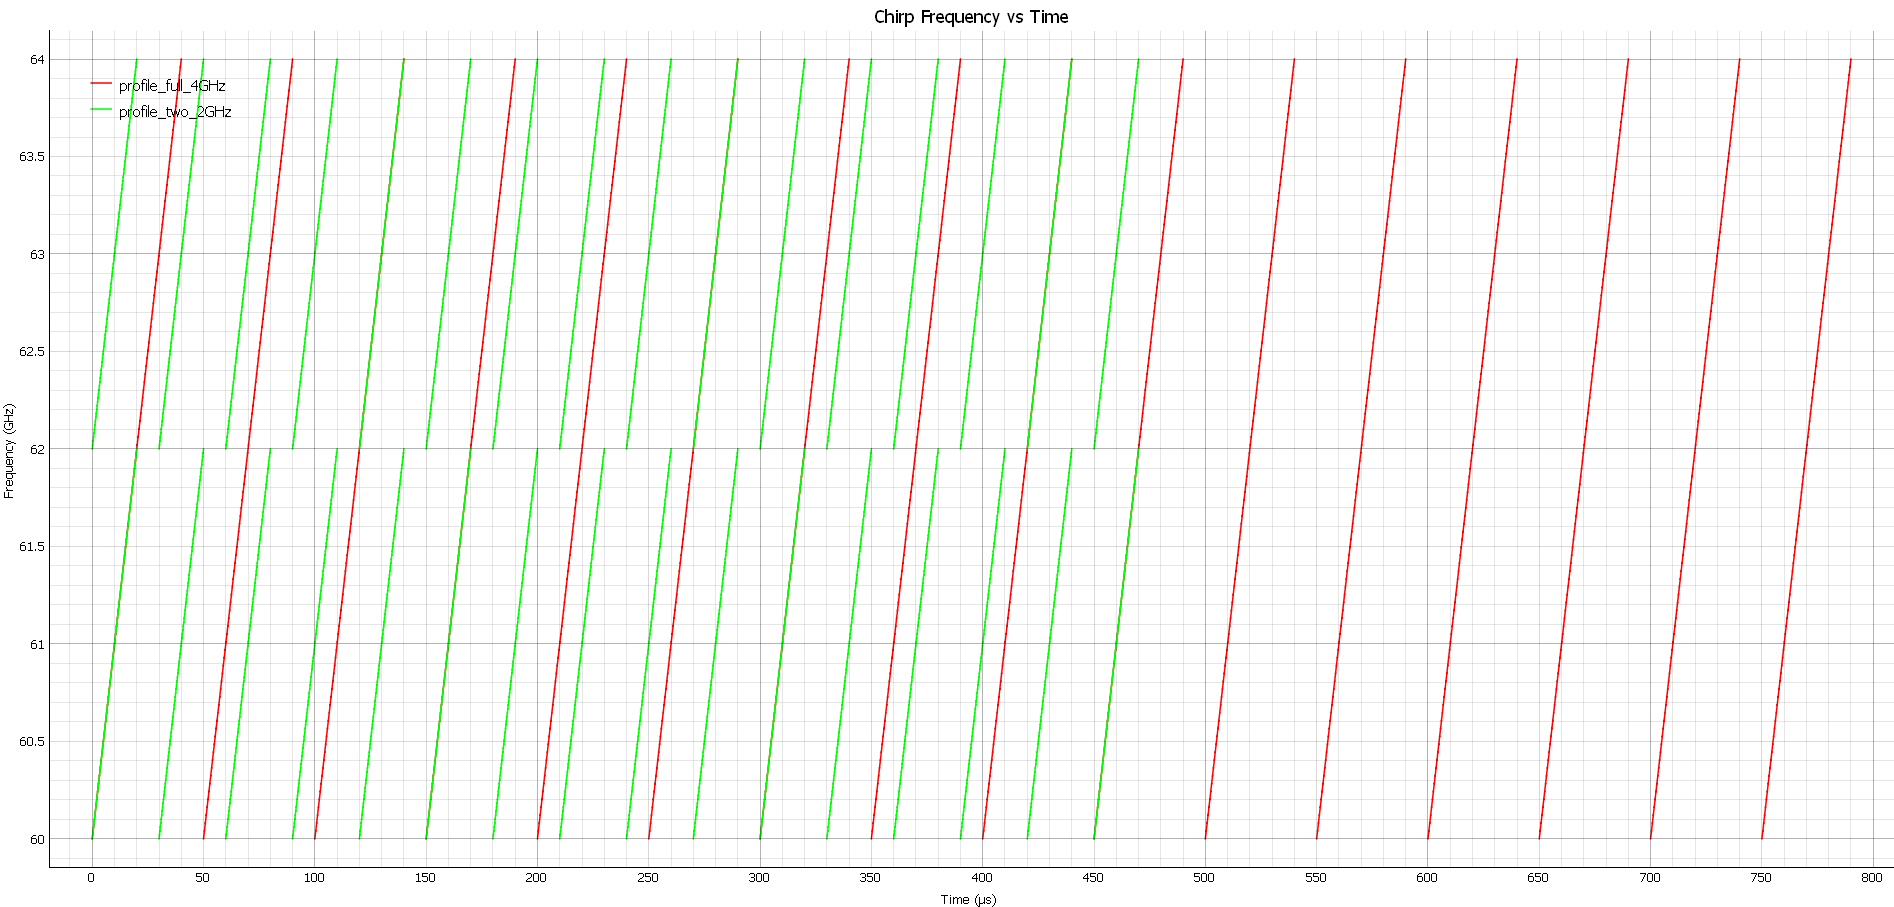
\includegraphics[width=1.0\linewidth]{images/profile_full_4GHz_2GHz.png}
    \caption{Overlay of single 4~GHz chirp and two 2~GHz chirps.}
    \label{fig:profile2And4GHz}
\end{figure}

{\small
\textit{Conclusion:} Best suited for ego-motion and odometry applications.
Can support multi-device environments with careful planning.
}

\begin{table}[h]
    \centering
    \caption{Comparison of Chirp Configuration Strategies}
    \label{tab:chirp_comparison}
    \resizebox{\columnwidth}{!}{%
    \begin{tabular}{|p{3.5cm}|p{3.2cm}|p{3.5cm}|p{3.8cm}|}
        \hline
        \textbf{Chirp Strategy} & \textbf{Range Resolution} & \textbf{Velocity Resolution} & \textbf{Best Use Case} \\
        \hline
        Full-Bandwidth Chirp (4 GHz) &
        High (Fine $\Delta R$) &
        Moderate (Few chirps/frame) &
        Precise mapping in single-radar setups; spatial accuracy prioritized \\
        \hline
        Divided-Band Chirps (e.g., 2×2 GHz) &
        Moderate (per chirp), improved via averaging &
        Moderate to High (more chirps/frame possible) &
        Robust odometry in noisy or multi-radar environments \\
        \hline
        Mixed Chirp Strategy (Full + Narrow) &
        High (from full chirp), plus enhanced Doppler &
        High (from multiple narrow chirps) &
        Ego-motion estimation; combines benefits of both range and Doppler precision \\
        \hline
    \end{tabular}%
    }
\end{table}

\vspace{1em}

The table above summarizes the key performance characteristics and use cases for each chirp configuration strategy.

The Full-Bandwidth Chirp maximizes spatial resolution, making it ideal for scenarios where high-fidelity mapping of nearby static objects is required—such as indoor SLAM or obstacle-rich environments. 
However, its wide spectral footprint and high ADC demand make it less suitable in systems where multiple radar devices operate simultaneously, as mutual interference becomes likely.
The Divided-Band Chirp approach offers a middle ground.
By allocating portions of the spectrum to separate chirps, it reduces system load and provides flexibility in processing. 
While individual chirps have lower range resolution, combining information across them improves detection stability. This strategy excels in distributed radar systems, such as in collaborative or multi-node sensor networks, where frequency coordination helps reduce ghost targets and interference.
Finally, the Mixed Chirp Strategy integrates the strengths of both previous approaches. 
A full-band chirp ensures accurate spatial anchoring, while narrow-band chirps provide temporal and Doppler refinement. 
This makes it the most adaptive option for applications like ego-motion estimation, where both precise localization and motion cues are critical. 
Its complexity, however, demands a more advanced signal processing pipeline and careful calibration to ensure synchronization between chirps.

In multi-radar environments, especially in close proximity (e.g., autonomous fleets or dual-radar vehicles), selecting chirp strategies that reduce spectral overlap is essential. Techniques like time-division multiplexing, slope diversity, and chirp staggering become critical tools to mitigate false detections and interference.

\vspace{1em}

\subsection{Chirp Configuration for Multi-Radar Systems}
\label{sec:chirp-multiradar}

When deploying multiple radar devices (e.g., front-left, front-right), interference becomes a significant challenge.
Simultaneous transmission using overlapping chirp frequencies can lead to ghost detections, false targets, and degraded signal-to-noise ratio. 
This due to the radio waves that are transmitter can cause collitions between each other creating this "ghost detections".
There are some strategies that can be employed to avoid this phenomenom.

\textbf{Recommended strategies:}
\begin{itemize}
    \item Use \textbf{non-overlapping frequency ranges} per device (e.g., 60–62~GHz on left, 62–64~GHz on right).
    \item Apply \textbf{interleaved chirps} in time: stagger chirps across sensors.
    \item Utilize \textbf{different slope values}: reduces likelihood of constructive interference.
    \item Match chirp \textbf{idle times} to ensure orthogonality.
\end{itemize}

These methods are essential to avoid ghost detections and preserve spatial coherence across sensors.

\vspace{1em}

{\small
\textit{Conclusion:} Chirp configuration in multi-radar environments requires trade-offs between resolution and isolation.  
Design must ensure orthogonality to avoid mutual interference.
}

\vspace{1em}

\subsection{Summary}

The configuration of chirps in FMCW radar defines its core capabilities in range and velocity estimation.
Depending on the target application — whether precision mapping, ego-motion tracking, or multi-device deployment — the choice of chirp bandwidth, duration, slope, and sequencing must be carefully made.

The following considerations are essential:
\begin{itemize}
    \item Use wide-band chirps when range precision is critical.
    \item Use many chirps with long frame durations when velocity resolution is prioritized.
    \item Use divided-band or mixed strategies in multi-radar systems to balance robustness and prevent interference.
\end{itemize}

Careful design enables robust radar odometry, reliable environment mapping, and scalable multi-radar systems.

%% \section{Theoretical Foundations: Mathematical Models and Algorithms for Radar-Based Object Detection}
%% \label{sec:Mathematical Models and Algorithms for Radar-Based Object Detection}

\section{Pipeline implementation: Modules implemented and mathematical explanation}
\label{sec:Mathematical Models and Algorithms for Radar-Based Object Detection}
As the radar sensor outputs its raw data in frames which contain a raw point cloud, a modular processing pipeline was developed.
This pipeline consists of different modules implementing the needed stages for pre-processing the sensor's data, filtering the point cloud, clustering and object detection.
The modular design allows the modification and adaption to different environments.
\par
In a pre-processing stage, the sensor's raw data frames, obtained via UART, are decoded and translated into frames containing individual points in a usable format with information about their $x,y,z,v_{r}$ and $SNR$ values.
They are then passed into a "Frame Aggregator" which stores a certain amount of frames in order to supply the later stages with the data from multiple frames and thus compensate for possible data sparsity.
The aggregated data is filtered by multiple filtering stages, starting with static parameters for the spatial dimension and the SNR, followed by a dynamic filtering stage using a comparison of the vehicle's estimated self-speed to the points' speeds for filtering.
The filtered points are then clustered using a two-stage approach and forwarded to the brake controller for object detection. The reason for the 2 stages of clustering is that for any given object that may be detected there would be noise or segmentation caused by some space between objects. So this 2 stages help us discard information that could be just a reflection and focus into the points that are considered as objects. This being done by having a permissive first stage, and afterwards a strict clustering stage to be able to label an object with a cluster ID for further processing.
\begin{figure}[!htbp]
    \centering
    \resizebox{0.48\textwidth}{!}{
        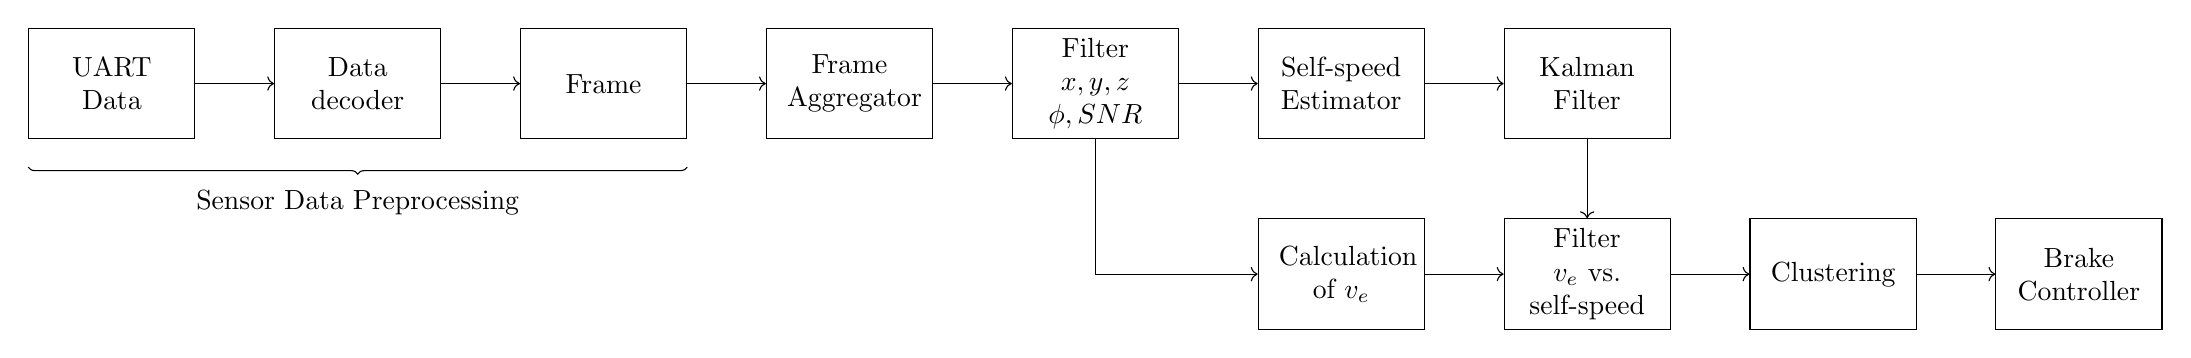
\begin{tikzpicture}
            % Block styles
            \tikzstyle{block} = [rectangle, draw, text width=4.5em, text centered, minimum width=6em, minimum height=4em]
            \tikzstyle{block_dashed} = [rectangle, draw, text width=2em, text centered, minimum width=4em, minimum height=4em, dashed]
            % Input and output
            \node[block] (uart) {UART\\Data};
            \node[block, right=of uart] (decoder) {Data decoder};
            \node[block, right=of decoder] (frames) {Frame};
            \node[block, right=of frames] (frame_aggr) {Frame\\Aggregator};
            \node[block, right=of frame_aggr] (coord_filter) {Filter\\$x,y,z$\\$\phi,SNR$};
            \node[block, right=of coord_filter] (self_speed_estim) {Self-speed Estimator};
            \node[block, right=of self_speed_estim] (self_speed_kalman) {Kalman Filter};
            \node[block, below=of self_speed_estim] (ve_speed_calc) {Calculation\\of $v_{e}$};
            \node[block, right=of ve_speed_calc] (ve_filter) {Filter\\$v_{e}$ vs. self-speed};
            \node[block, right=of ve_filter] (clustering) {Clustering};
            \node[block, right=of clustering] (brake_controller) {Brake\\Controller};
            % Connections
            \draw[->] (uart) -- (decoder);
            \draw[->] (decoder) -- (frames);
            \draw[->] (frames) -- (frame_aggr); % Connection from antenna to RF amplifier
            \draw[->] (frame_aggr) -- (coord_filter);
            \draw[->] (coord_filter) -- (self_speed_estim);
            \draw[->] (coord_filter.south) |- (ve_speed_calc.west);
            \draw[->] (self_speed_estim) -- (self_speed_kalman);
            \draw[->] (self_speed_kalman) -- (ve_filter);
            \draw[->] (ve_speed_calc) -- (ve_filter);
            \draw[->] (ve_filter) -- (clustering);
            \draw[->] (clustering) -- (brake_controller);

            \draw [decorate, decoration = {brace, mirror, raise=10pt}] (uart.south west) --  (frames.south east) node[pos=0.5,below=15pt,black]{Sensor Data Preprocessing};
        \end{tikzpicture}
    }
    \caption{Block diagram of the pipeline}
    \label{fig:block_diag_pipeline}
\end{figure}

\FloatBarrier\noindent

%\begin{figure}[!htbp]
%    \centering
%    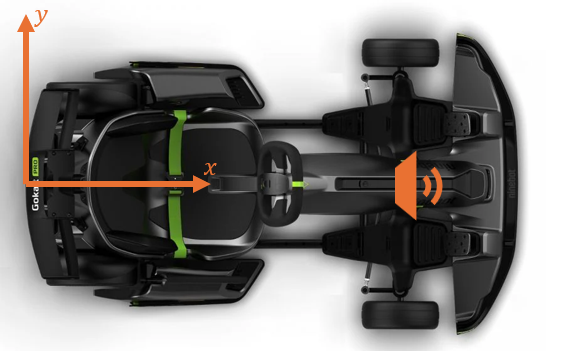
\includegraphics[width=1.0\linewidth]{images/ninebot.png}
%    \caption{Schematic sensor distribution}
%    \label{fig: One sensor is located in the front of the test vehicle}
%\end{figure}
%\FloatBarrier\noindent
\subsection{Sensor Coordinate Transformations}
\label{subsec:transformations}

Each radar sensor in the dual-radar configuration is physically mounted with a specific orientation and tilt relative to the vehicle's forward direction. 
To ensure a common frame of reference for all points, it is necessary to compensate for:

\begin{itemize}
    \item \textbf{Yaw rotation}: due to angled placement (±30$^\circ$) of the radar modules.
    \item \textbf{Pitch tilt}: due to upward mounting tilt (15$^\circ$), which must be compensated to recover horizontal geometry.
    \item \textbf{Sensor offset}: due to the physical separation of the radar sensors in the horizontal axis (X-axis).
\end{itemize}

A yaw rotation \( R_{\text{yaw}} \) was first implemented, followed by a pitch correction \( R_{\text{pitch}} \), and finally a translation vector \( \vec{t} \) was applied to account for the physical position of the sensors with respect to the vehicle's coordinate origin.

The full transformation can be expressed as:

\begin{equation}
T_{\text{veh}} = R_{\text{yaw}} \cdot R_{\text{pitch}} \cdot \vec{p}_{\text{radar}} + \vec{T}
\label{eq:radar_to_vehicle_transform}
\end{equation}

Where:
\begin{itemize}
    \item \( \vec{p}_{\text{radar}} \) is a radar point in sensor coordinates.
    \item \( R_{\text{yaw}} \) is a 2D or 3D rotation around the vertical axis.
    \item \( R_{\text{pitch}} \) corrects for the upward sensor tilt.
    \item \( \vec{T} \) is the translation vector.
\end{itemize}

\vspace{1em}

Let $(x, y, z)$ be the original point from the radar frame, with $x$ to the right, $y$ forward, and $z$ upward. 
The transformations applied are as follows:

\paragraph{Yaw Correction (Z-axis Rotation)}
The radar sensors are rotated relative to the vehicle frame:

\begin{itemize}
    \item Radar A (Left): Mounted at $+30^\circ$ yaw $\Rightarrow$ compensated with $-30^\circ$ rotation.
    \item Radar B (Right): Mounted at $-30^\circ$ yaw $\Rightarrow$ compensated with $+30^\circ$ rotation.
\end{itemize}

The 2D rotation in the XY-plane is defined as:
\[
\begin{bmatrix}
x' \\
y'
\end{bmatrix}
=
\begin{bmatrix}
\cos(\theta) & -\sin(\theta) \\
\sin(\theta) & \cos(\theta)
\end{bmatrix}
\begin{bmatrix}
x \\
y
\end{bmatrix}
\]

where $\theta = \pm30^\circ$ depending on the sensor.

\begin{figure}[!htbp]
    \centering
    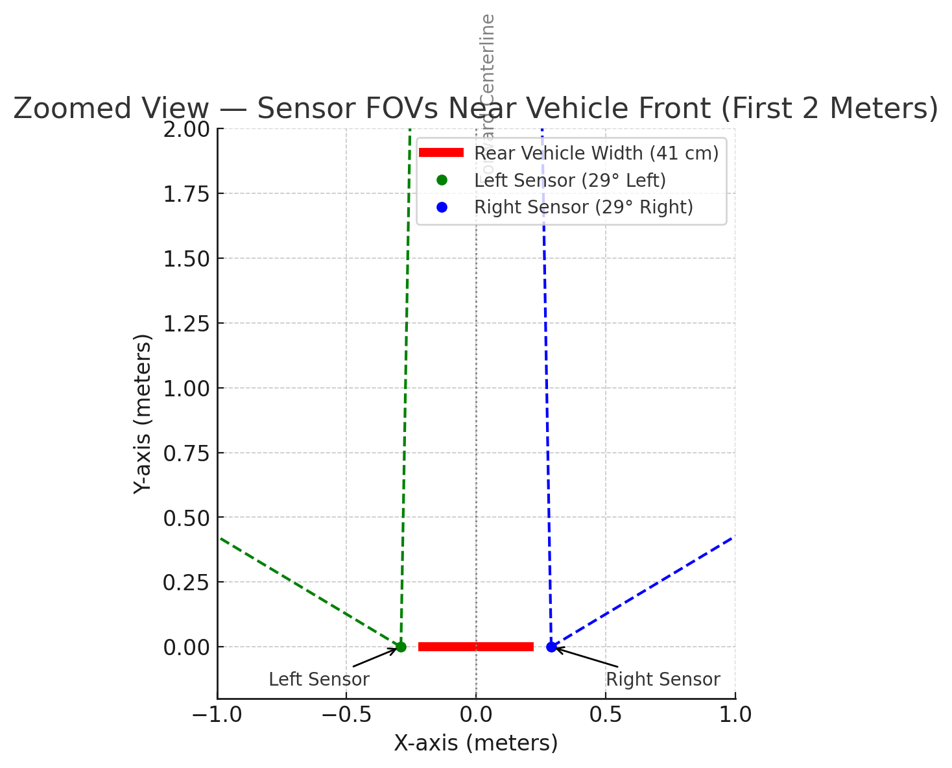
\includegraphics[width=0.8\linewidth]{images/SensorsRotation.png}
    \caption{Yaw rotation of sensors around the Z-axis (±30$^\circ$).}
    \label{fig:z_axis_rotation}
\end{figure}

\vspace{2em}

\paragraph{Pitch Compensation (X-axis Rotation)}
Since the radar sensors are tilted upward by $15^\circ$, a corrective rotation around the X-axis is applied to bring the points back to a horizontal perspective: 

\[
\begin{bmatrix}
x'' \\ y'' \\ z''
\end{bmatrix}
=
\begin{bmatrix}
1 & 0 & 0 \\
0 & \cos(\phi) & -\sin(\phi) \\
0 & \sin(\phi) & \cos(\phi)
\end{bmatrix}
\begin{bmatrix}
x' \\ y' \\ z
\end{bmatrix}
\]

where $\phi = -15^\circ$ (negative to reverse the upward tilt).

\begin{figure}[!htbp]
    \centering
    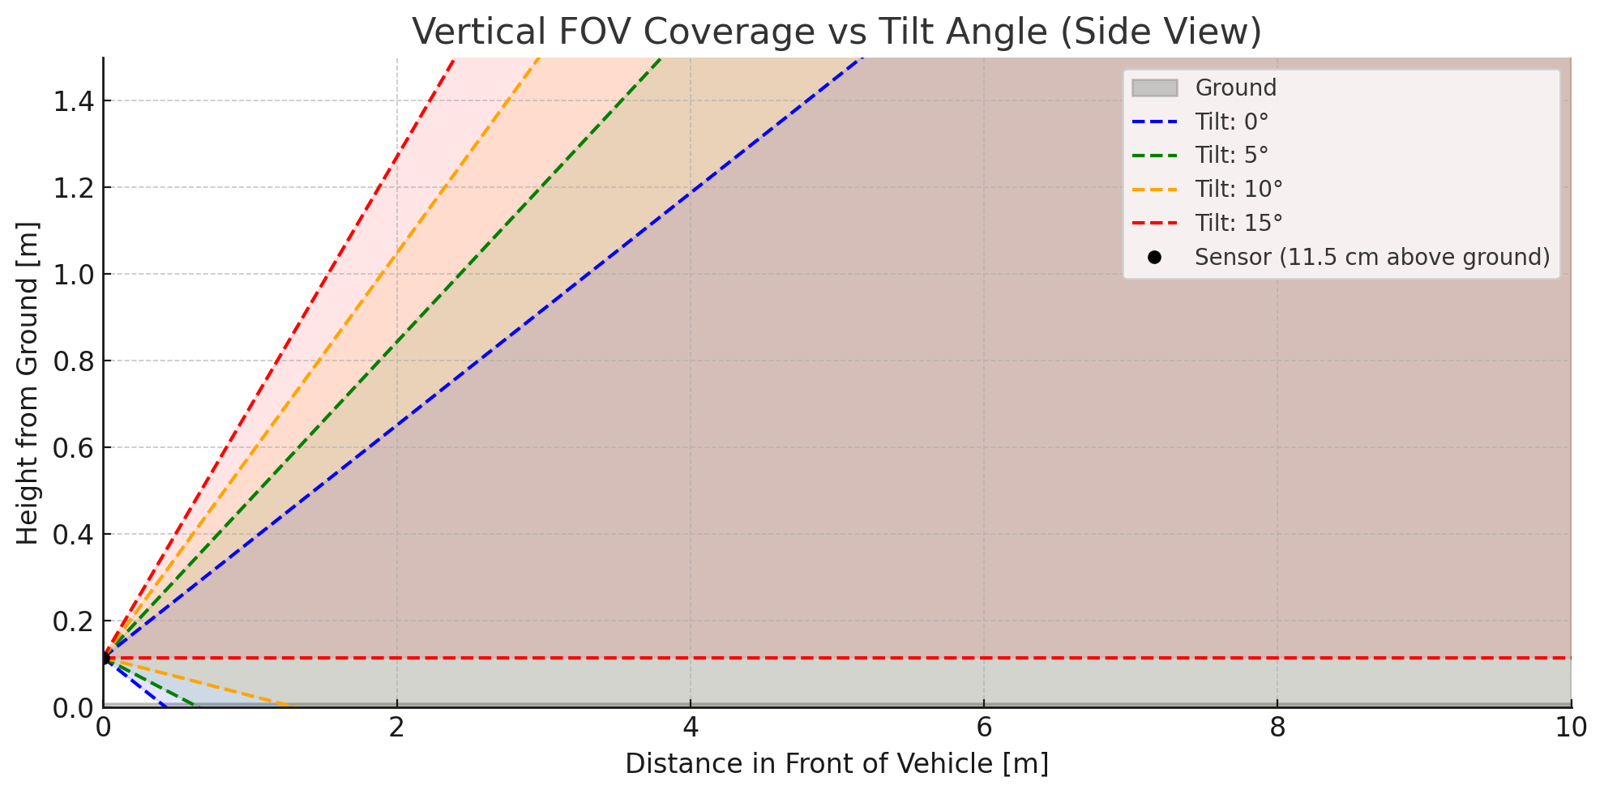
\includegraphics[width=0.8\linewidth]{images/TiltSensor.png}
    \caption{Pitch compensation for $15^\circ$ upward tilt.}
    \label{fig:x_axis_rotation}
\end{figure}

\vspace{2em}

\paragraph{X-Axis Offset Compensation}
After rotation, each sensor's point cloud was translated along the X-axis to align with the vehicle's center:
\begin{itemize}
    \item Radar A: $x \leftarrow x - 0.32$ meters
    \item Radar B: $x \leftarrow x - 0.28$ meters
\end{itemize}

This translation ensured both sensors were aligned in a common vehicle-centric frame.

\begin{figure}[!htbp]
    \centering
    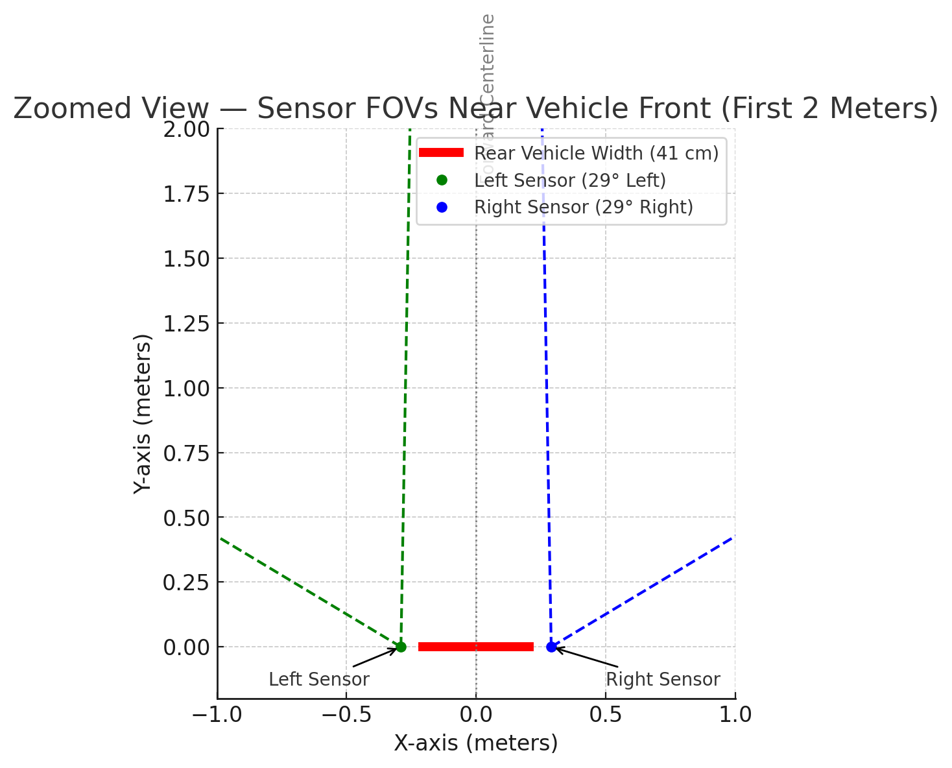
\includegraphics[width=0.8\linewidth]{images/RotationSensor.png}
    \caption{Final extrinsic configuration combining yaw, pitch, and translation.}
    \label{fig:extrinsics}
\end{figure}

\vspace{2em}

\paragraph{Impact of Transformations on Point Clouds}
The importance of these corrections becomes evident when comparing raw and transformed data. Without transformations, detections from the left and right radars appear misaligned, producing duplicated or inconsistent clusters. After applying yaw, pitch, and translation compensation, the fused point cloud exhibits coherent structures, with static landmarks consistently overlapping across sensors.

Figures~\ref{fig:dualSensorCalib_2mts}--\ref{fig:AFTERdualSensorCalibRANSAC_2mts} illustrate this process, showing raw point clouds, clustered representations, and RANSAC fits before and after calibration. The transformed data serves as a stable basis for subsequent steps in the odometry pipeline, such as ICP-based submap alignment.

\begin{figure}[!htbp]
    \centering
    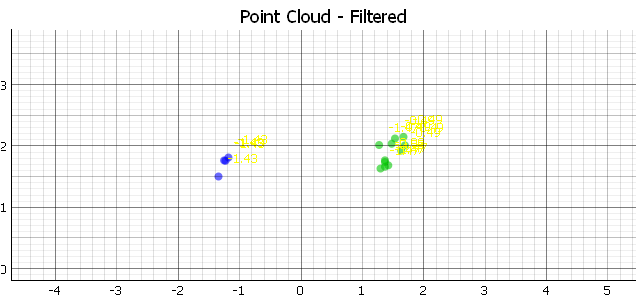
\includegraphics[width=0.9\linewidth]{images/dualSensorCalib_2mts.png}
    \caption{Raw dual-sensor point cloud before geometric transformations.}
    \label{fig:dualSensorCalib_2mts}
\end{figure}

\begin{figure}[!htbp]
    \centering
    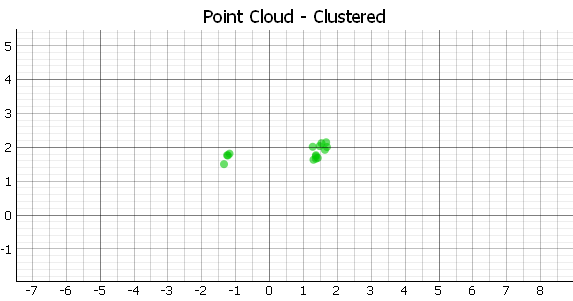
\includegraphics[width=0.9\linewidth]{images/dualSensorCalibCluster_2mts.png}
    \caption{Clustered detections from both radars before transformation.}
    \label{fig:dualSensorCalibCluster_2mts}
\end{figure}

\begin{figure}[!htbp]
    \centering
    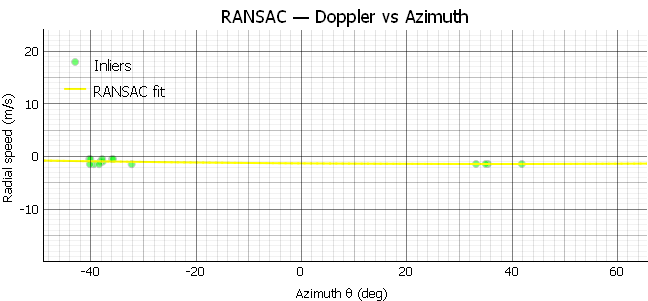
\includegraphics[width=0.9\linewidth]{images/dualSensorCalibRANSAC_2mts.png}
    \caption{RANSAC fit on Doppler velocities before transformation.}
    \label{fig:dualSensorCalibRANSAC_2mts}
\end{figure}

\begin{figure}[!htbp]
    \centering
    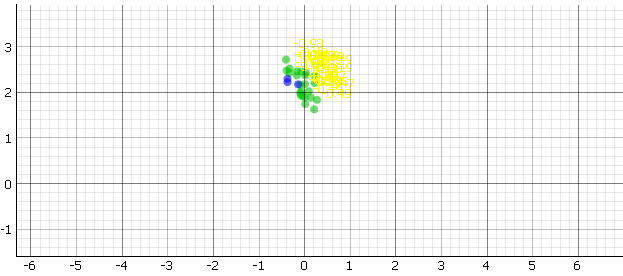
\includegraphics[width=0.9\linewidth]{images/AFTERdualSensorCalib_2mts.png}
    \caption{Fused point cloud after geometric transformations.}
    \label{fig:AFTERdualSensorCalib_2mts}
\end{figure}

\begin{figure}[!htbp]
    \centering
    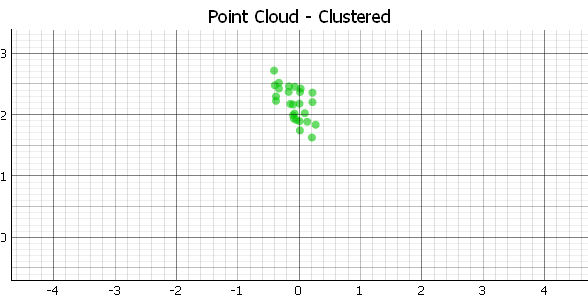
\includegraphics[width=0.9\linewidth]{images/AFTERdualSensorCalibCluster_2mts.png}
    \caption{Clustered detections after transformation, showing improved alignment.}
    \label{fig:AFTERdualSensorCalibCluster_2mts}
\end{figure}

\begin{figure}[!htbp]
    \centering
    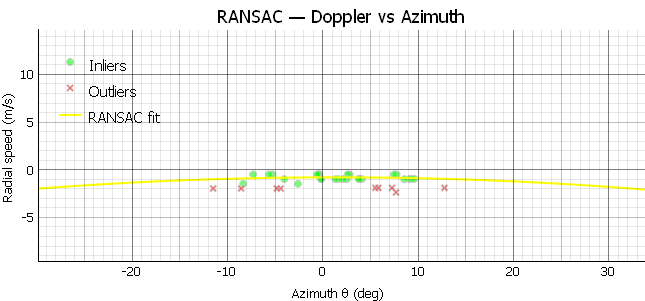
\includegraphics[width=0.9\linewidth]{images/AFTERdualSensorCalibRANSAC_2mts.png}
    \caption{RANSAC fit on Doppler velocities after transformation.}
    \label{fig:AFTERdualSensorCalibRANSAC_2mts}
\end{figure}

\vspace{1em}

\paragraph{Summary of Extrinsics}
\begin{itemize}
    \item \textbf{Left radar:} yaw $+30^\circ$, pitch $-15^\circ$, translation $(-0.32, 0, 0)$.
    \item \textbf{Right radar:} yaw $-30^\circ$, pitch $-15^\circ$, translation $(-0.28, 0, 0)$.
\end{itemize}

This extrinsic calibration ensures that dual-radar data is expressed in a coherent vehicle-centric frame, which is critical for downstream modules such as clustering, odometry, and obstacle tracking.


\subsection{Frame Aggregator}
\label{sec:Frame Aggregator}
The decoded frames are passed into a frame aggregator stage as a first step, which utilizes data aggregation to reduce possible data sparsity of individual frames. 
Data aggregation involves combining multiple consecutive data sets to create a more comprehensive and reliable dataset for processing. This approach increases both useful information and noise, but ultimately enhances the quality of radar point clouds for object detection and tracking stability.
For point clouds from radar sensors, aggregating multiple frames enhances data consistency and density, improving the system’s ability to reconstruct objects and detect motion patterns.

\subsubsection{Single Frame}
Using radar point cloud data from a single frame has inherent limitations, which can lead to incomplete or misleading detections:
\begin{itemize}
    \item A single frame may not capture enough points, leading to failed detections or incomplete object reconstruction.
    \item Limited point data can cause objects to appear fragmented or indistinguishable from noise.
\end{itemize}

\begin{figure}[!htbp]
    \centering
    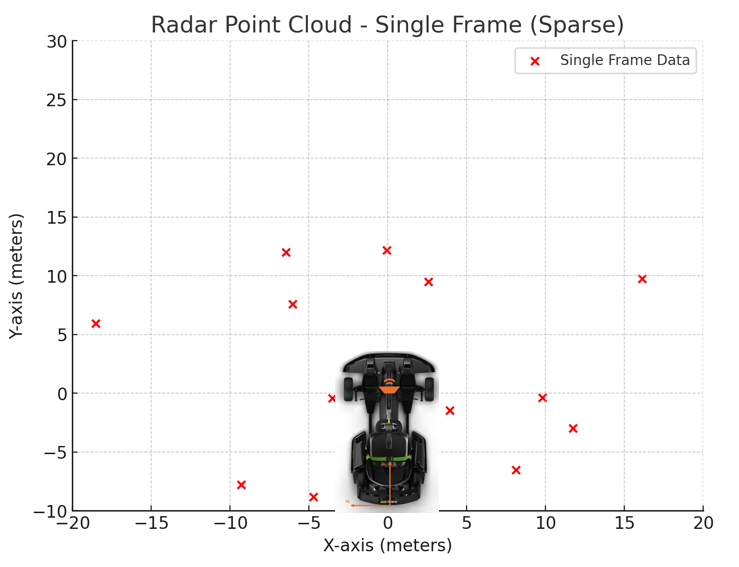
\includegraphics[width=0.5\linewidth]{images/singleframe.png}
    \caption{Single Frame visualization.}
    \label{fig: Single Frame visualization}
\end{figure}

Consequently, it is difficult to precisely rebuild or map complex objects due to the limited points in the point cloud and information contained in a single radar frame, which results in ambiguity and uneven detection performance.
This ambiguity can result in the erroneous detection of a large object or the merging of two different objects into one, as the clustering or detection algorithm may malfunction, not due to inherent flaws in the algorithm itself, but rather due to the inherent flaws in the data. This phenomenon occurs when two or more objects are in close proximity from each other, but can not be distinguished from each other because of the lack of points in a single frame.

To mitigate these issues, frame aggregation can be leveraged, an approach supported by the Law of Large Numbers (LLN). By accumulating multiple frames, the impact of random variations can be reduced, such as:
\begin{equation}
    \frac{\sigma^2}{N}
    \label{eq:variance_per_sample_size}
\end{equation}
This leads to a more statistically stable representation of objects; which means that the larger the sample is, the less effect the noise will have. Additionally, variance reduction helps to filter out erroneous detections while improving the reliability of motion estimation.

\subsubsection{Multiple Frames}
In contrast, the aggregation of multiple frames can significantly enhance object detection capabilities.
Using this technique the algorithm can be tricked, by making it believe that there is more information that it was actually obtained from the single frame. This comes with the drawback that there will be some older data inside the processed frame.
\begin{figure}[!htbp]
    \centering
    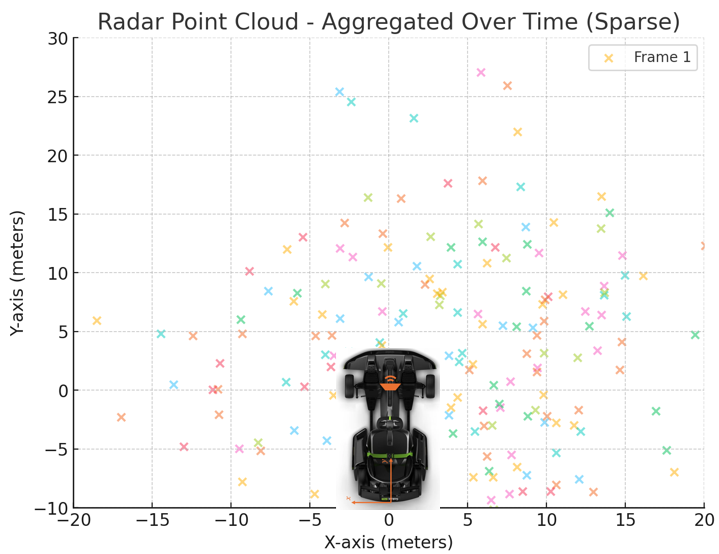
\includegraphics[width=0.5\linewidth]{images/multiframe.png}
    \caption{Frame Aggregation visualization.}
    \label{fig: Frame Aggregation visualization}
\end{figure}

This aggregation approach improves the accuracy of velocity and trajectory estimations, strengthens object identification's resilience against transient noise, and reduces problems related to sparse data.
It was implemented by using a stack with a fixed size, executing a "pop" operation prior to the insertion of the new frame at the stack's end.
The point cloud containing the points of all frames stored in the frame aggregator is then passed to the next stage.
\subsection{x,y,z,SNR Filter}
The point cloud's points are passed through a first static filtering stage to remove points caused by noise, clutter or targets outside of the area of interest before being used for further processing.
This static filtering stage consists of four different filters, filtering out points by different attributes:
\begin{enumerate}
    \item Filtering by $SNR$: All points with a $SNR$ lower than \SI{12}{\deci\bel} are filtered out to remove points with a low signal and those that might be caused by noise or clutter.
    \item Filtering by $z$ coordinate: All points below a $z$ value of \SI{0}{\meter} and above \SI{2}{\meter} are filtered out to remove points caused by the ground or the ceiling.
    \item Filtering by $y$ coordinate: All points below a $y$ value of \SI{0.3}{\meter} are filtered out to remove points created by the driver's feet.
    \item Filtering by $\phi$: All points with an azimuth bigger than \SI{85}{\degree} are filtered out to remove points that are outside the area of interest.
\end{enumerate}
\textit{Note: The origin of the points' coordinate system is the sensor itself, so a coordinate of $(\SI{0}{\meter},\SI{0}{\meter},\SI{0}{\meter})$ is essentially at the sensor's mounting position and therefore approx. \SI{0.3}{\meter} above the ground.}
\par
As the static filtering stage only keeps points which are relevant in terms of there spatial position and $SNR$ for the following stages, it effectively decreases the computation time of each frame and prevents the following stages from processing invalid data.
The filtered point cloud is then passed to the next stages, the self-speed estimator and the dynamic filtering stage.

\begin{figure}[!htbp]
\centering
\begin{subfigure}{0.24\textwidth}
  \centering
  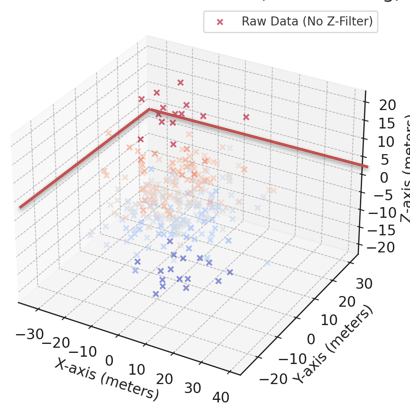
\includegraphics[width=\textwidth]{images/No_filter.png}
  \caption{Input}
\end{subfigure}
\begin{subfigure}{0.24\textwidth}
  \centering
  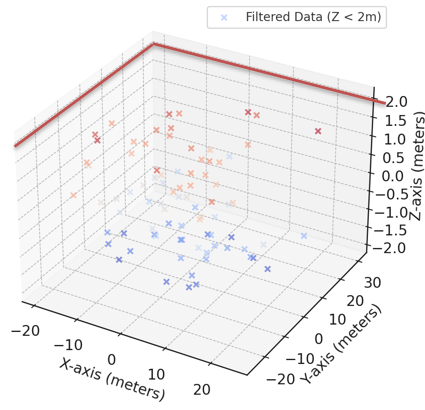
\includegraphics[width=\textwidth]{images/filter.png}
  \caption{Output}
\end{subfigure}
\caption{Example visualization of the input and output when filtering by the value of the $z$ coordinate.}
\label{fig:static_filter_z_example}
\end{figure}
\FloatBarrier\noindent



\subsubsection{Static vs Non-static objects}
In the detected data there will always be static or moving objects in the field of view, this is more prominent when the sensor is mounted in a moving frame.
In this case every thing is moving from the perspective of the sensor, so how does the differentiation happens to identify statis vs non-static objects, this is simple, by leveraging on the doppler effect concept.
Using the doppler effect and understanding it is crutial for this step, as it is what will allow the algorithm to focuse the processing only in the static targets that are detected.

In this case, making the assumption that the sensor is mounted in a vehicle that goes 2 meters per second. With this in consideration, the assumption that all static targets should have a radial speed similar to the 2 meters per second.
This speed cannot be the same as the angle of detection can affect, the accuracy that may be obtained through the chirp configuration, etc.
Multiple variables can be added into this "equation", but the assumption that the static targets measured radial speed is close to the vehicle speed we can know which target to keep and which target to discard with only this paramter.

However that leaves us with the problem of how to group such targets. At this point the RANSAC algorithm becomes useful, as it will do the grouping for us, by ussing the radial speed.

\section{RANSAC-Based Motion Filtering}

To differentiate static and dynamic objects in the radar point cloud, we use a RANSAC-based approach on the relationship between azimuth angle $\theta$ and radial Doppler velocity $v_d$.

\subsection*{Principle}
Under ideal conditions, static objects exhibit Doppler values consistent with the vehicle's own motion and orientation. 
These values follow a smooth curve when plotted against azimuth. 
Moving objects, however, deviate from this pattern.
RANSAC (Random Sample Consensus) is used to robustly fit a model to the expected Doppler pattern of static objects. 
Points that do not conform to the model are classified as dynamic.

\subsection*{Mathematical Model}

We assume a second-degree polynomial relationship:
\[
v_d = a\theta^2 + b\theta + c
\]

RANSAC fits this model by iteratively:
\begin{itemize}
    \item Sampling minimal subsets of the data,
    \item Fitting the polynomial,
    \item Identifying inliers whose residual error is below a threshold,
    \item Selecting the model with the highest consensus.
\end{itemize}

Let $\mathbf{X}$ be the input azimuth values and $\mathbf{y}$ the Doppler speeds:

\[
\mathbf{X} = \begin{bmatrix} \theta_1 \\ \theta_2 \\ \vdots \\ \theta_n \end{bmatrix}, \quad 
\mathbf{y} = \begin{bmatrix} v_{d1} \\ v_{d2} \\ \vdots \\ v_{dn} \end{bmatrix}
\]

RANSAC estimates polynomial coefficients $\mathbf{w} = [a, b, c]^T$ such that:

\[
\mathbf{y} \approx \Phi(\mathbf{X}) \cdot \mathbf{w}, \quad
\Phi(\mathbf{X}) = 
\begin{bmatrix}
\theta_1^2 & \theta_1 & 1 \\
\theta_2^2 & \theta_2 & 1 \\
\vdots & \vdots & \vdots \\
\theta_n^2 & \theta_n & 1 \\
\end{bmatrix}
\]

\subsection*{Use in Pipeline}

This filtering step occurs after point-wise filtering (e.g., Doppler and range cuts). It outputs:
\begin{itemize}
    \item \textbf{Inliers} – points likely to be static (used in clustering/ICP)
    \item \textbf{Outliers} – likely dynamic, excluded from ego-motion estimation
\end{itemize}

%TODO: Fix image, use one from project.
\begin{figure}[!htbp]
    \centering
    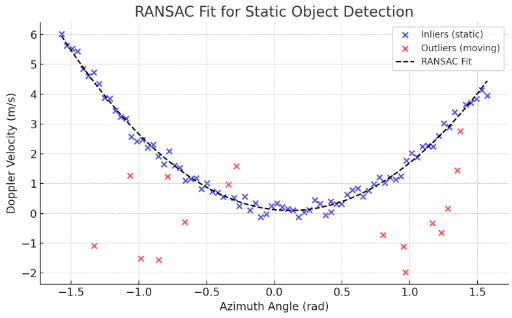
\includegraphics[width=1.0\linewidth]{images/RANSAC.png}
    \caption{RANSAC fit of Doppler vs. azimuth. Inliers = static (blue), Outliers = moving (red)}
    \label{fig:ransac_static_dynamic}
\end{figure}

\subsection{Static vs Dynamic Objects: Role of Doppler}

In radar-based perception, identifying dynamic objects (e.g., vehicles, pedestrians) amidst a cluttered scene of static structures (e.g., walls, poles) is critical.
This task becomes more complex when the radar is mounted on a moving platform, such as a vehicle.
From the sensor's perspective, **all objects appear to move** due to its own motion. The key to resolving this ambiguity lies in leveraging the **Doppler effect**.
The Doppler effect describes how the observed frequency of a wave changes based on the relative motion between the source and the observer. For radar systems, this translates into measurable **radial velocity** values: the component of an object's velocity along the line of sight of the radar.
Assuming the vehicle is moving at a constant speed (e.g., 2 m/s), static targets—such as buildings or parked cars—should exhibit Doppler values that align with this ego-motion, adjusted by their detection angle (azimuth).
That is, a static object located directly ahead will have a Doppler value close to $+2$ m/s (if approaching), while an object at the side (90 azimuth) will have nearly 0 m/s radial velocity.
This expected Doppler pattern for static objects traces a smooth curve when plotted against azimuth. Deviations from this curve indicate potential dynamic objects with their own independent motion.
To robustly extract this pattern from noisy measurements, **RANSAC** is applied to fit a second-order polynomial to the Doppler vs. azimuth data. This model captures the expected distribution of static points.
Points that significantly deviate from this model are considered **dynamic** and excluded from ego-motion estimation steps.

\paragraph{Benefits of RANSAC-Based Filtering:}
\begin{itemize}
    \item Ignores noisy or misdetected points by considering consensus.
    \item Segregates the scene into static (inliers) and dynamic (outliers) segments.
    \item Improves the accuracy of clustering and motion estimation by focusing only on consistent, stationary targets.
\end{itemize}

The filtered result not only enables accurate **object tracking**, but also prevents false ego-motion estimates that could arise from moving targets dominating the point cloud.
\subsection{Self-speed Estimator}
\label{sec:self-speed_estimator}
The vehicle's self-speed is used for distinguishing between points of stationary and moving objects and filtering out the points of moving objects in a later block of the pipeline.
It therefore needs to be determined in a reliable way.
Traditional approaches usually utilize external sensors such as wheel encoders, Global Positioning System (GPS), or Inertia Measurement Units (IMUs).
In this project, a technique was developed that determines the vehicle's self-speed only by processing the point cloud's data.
An angle $\phi_{p}$ was defined between each individual point of the point cloud and the radar sensor's centerline:
\par
\begin{figure}[!htbp]
    \centering
    %\resizebox{0.48\textwidth}{!}{
        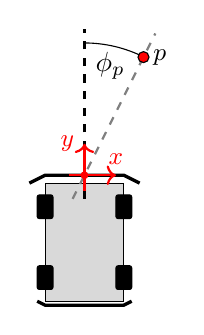
\begin{tikzpicture}
            \gokart{0}{0}{0}

            \coordinate(O) at (0,0);
            \coordinate(P) at (0.75,1.5);
            \coordinate(A) at (0,1.5);

            \draw[dashed, thick, gray] ($(P)!1.2!(O)$) -- ($(O)!1.2!(P)$);
            \draw[dashed, thick] ($(A)!1.2!(O)$) -- ($(O)!1.24!(A)$);
            \draw pic["$\phi_{p}$", draw=black, angle radius=1.68cm, angle eccentricity=0.85] {angle=P--O--A};
            \draw[fill=red] (P) circle (0.07) node [right] {\small $p$};

            \draw[->, thick, red] (-0.2,0) -- (0.4,0) node[above] {\small $x$};
            \draw[->, thick, red] (0,-0.2) -- (0,0.4) node[left] {\small $y$};
            \fill[red] (0,0) circle (0.05);
        \end{tikzpicture}
    %}
    \caption{Definition of the angle $\phi_{p}$}
    \label{fig:def_angle_phi}
\end{figure}
\FloatBarrier\noindent
These angles $\phi_{p}$ can be calculated using the points' cartesian position information:
\begin{equation*}
    \phi_{p} = arctan\left(\frac{x_{p}}{y_{p}}\right)
    \label{eq:calc_angle_phi}
\end{equation*}
A curve $v(\phi)$ is fitted through the points with their angles $\phi_{p}$ serving as the independent variable and their radial speeds $v_{r,p}$ as the dependent variable.
The curve's value $v(\phi = \SI{0}{\degree})$ then gives an estimation for the vehicle's self speed.
\par
This is possible because the perceived radial speed $v_{r,p}$ of a point related to a stationary target is dependent on the angle $\phi_{p}$ and follows a cosine when being passed at a certain speed $v_{0}$:
\begin{equation*}
    v_{r,p}(v_{0},\phi_{p}) = -v_{0} \cdot cos(\phi_{p})
\end{equation*}
At $\phi = \SI{0}{\degree}$, the radial speed is therefore equal to the vehicle's self speed.
Because there is rarely a point exactly at \SI{0}{\degree} and the radial speeds of the points also include noise, the approach uses all available points after the first filtering stage to fit a curve and effectively give the best possible estimation.
The implementation uses a least squares polynomial regression approach to fit a 2nd order polynomial (see \cite{numpy_polyfit}), which is sufficient in this case as the angle $\phi$ is defined in a way that $\phi_{p} = \left[-\frac{\pi}{2},\frac{\pi}{2}\right]$, so the cosine can be approximated by a 2nd order polynomial:
\begin{equation*}
    cos(\phi_{p}) \approx a \cdot \phi_{p}^2 + b \quad with\enspace \phi_{p} = \left[-\frac{\pi}{2},\frac{\pi}{2}\right]
\end{equation*}
Multiple runs of this algorithm with recorded test data proved the technique's principle.
\begin{figure}[!htbp]
    \centering
    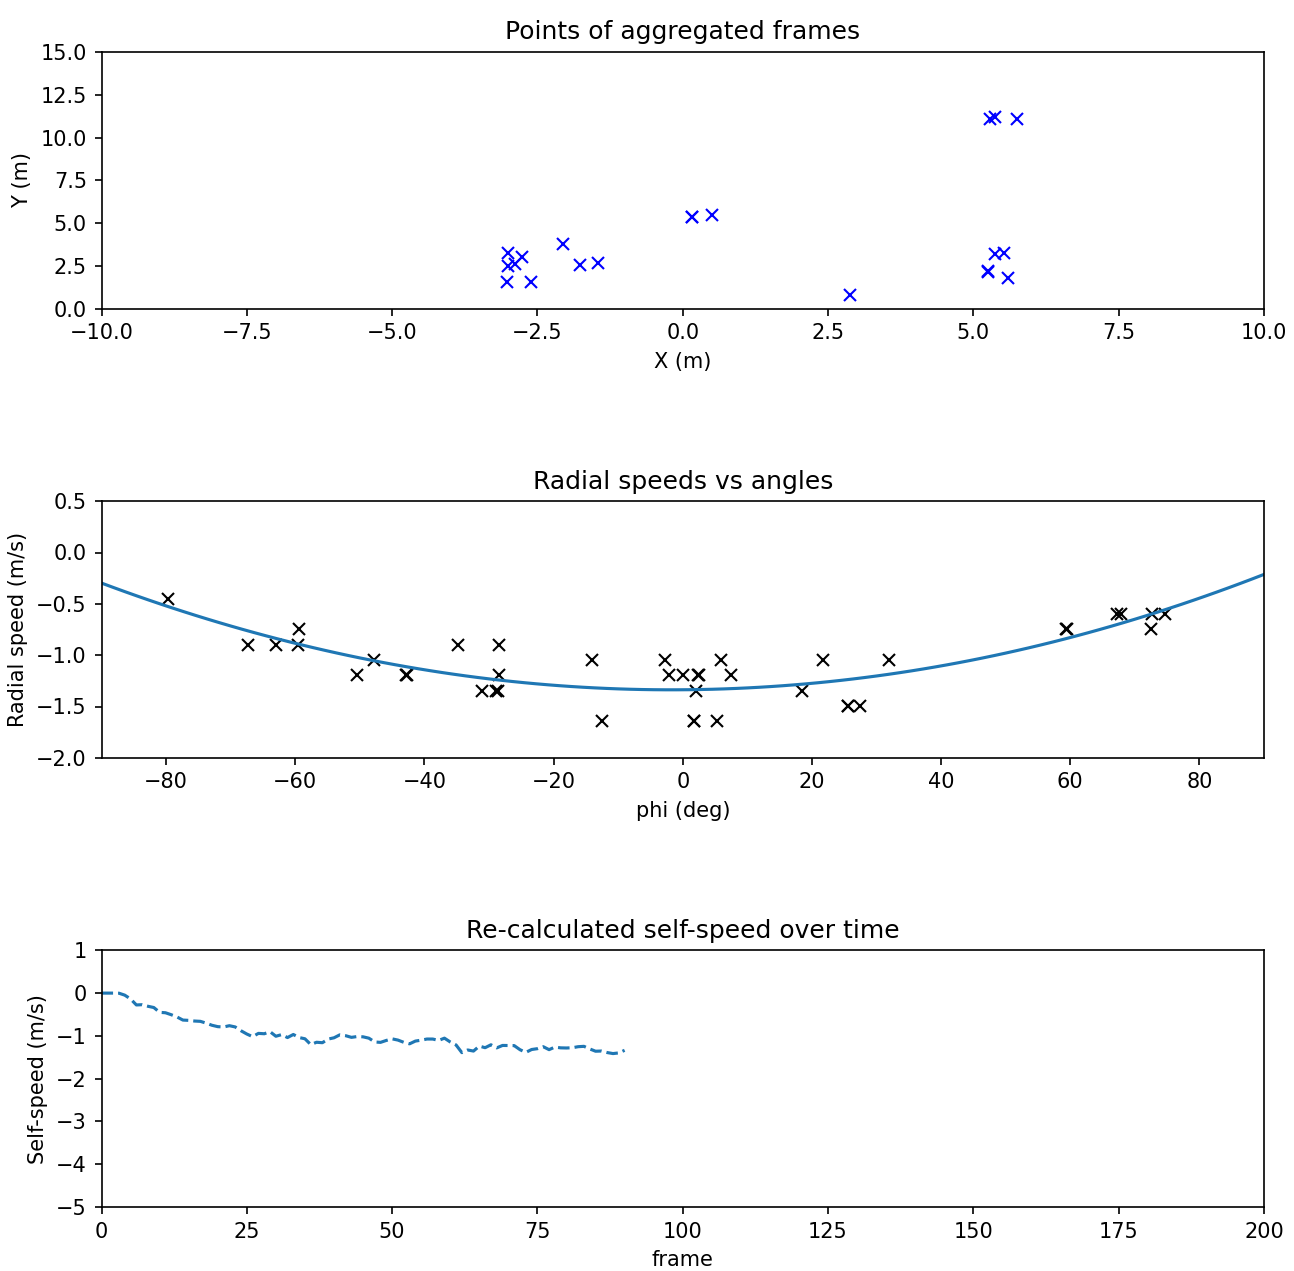
\includegraphics[width=1.0\linewidth]{images/self_speed_reality.png}
    \caption{Test run with recorded data and visualization.}
    \label{fig:self_speed_test_data}
\end{figure}
\FloatBarrier\noindent
During tests, the self-speed estimated by this technique matched the go-kart's built-in speed indicator with some small static offset but also showed heavy fluctuations from time to time when the radar sensor's output only contained a small amount of points.
Although this influence could be reduced by tuning the amount of frames stored in the frame aggregator, a stage containing a Kalman Filter was added after the self-speed estimation before the self-speed value is passed to the following pipeline blocks.



%% [20/03/2025] Leander: Rework done, commentend out bc. probably not needed anymore
%% ---------------------------------------
\begin{comment}

\todo {This whole chapter needs to be done again}
The estimation of a vehicle’s self-speed is a fundamental requirement for autonomous navigation and advanced driver-assistance systems (ADAS). Traditional methods often rely on external sensors such as wheel encoders, GPS, or IMUs to determine vehicle velocity. However, in this project, no external sensor was used for speed estimation. Instead, velocity was estimated exclusively using data from an mmWave radar sensor, leveraging its Doppler measurements to infer motion.

The proposed approach estimates ego-motion (velocity) of the vehicle by analyzing the radial velocity obtained from the radar point cloud. The mmWave radar measures the Doppler shift of each detected point, which corresponds to the relative velocity of objects with respect to the sensor. Assuming that all detected objects are static, the observed Doppler velocities can be directly attributed to the vehicle’s own motion.

\begin{figure}[!htbp]
    \centering
    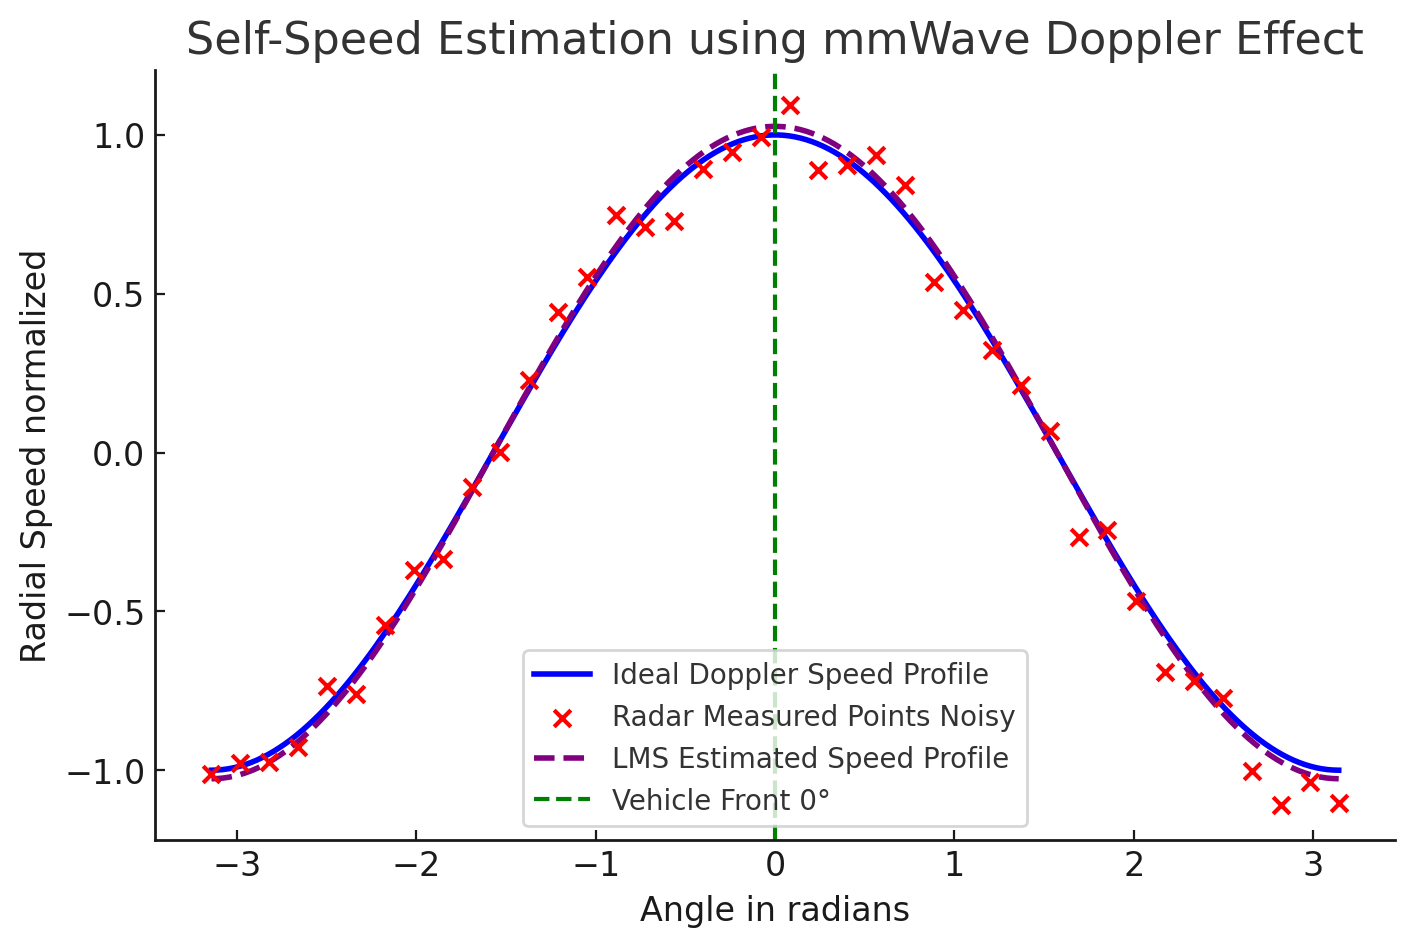
\includegraphics[width=1.0\linewidth]{images/Self_Speed_Doppler.png}
    \caption{Self-Speed Estimation Using MmWave Doppler Effect}
    \label{fig: Self-Speed Estimation Using MmWave Doppler Effect}
\end{figure}
\FloatBarrier\noindent
To estimate speed accurately, radial velocities are fitted to a cosine function that simulates the Doppler shift as a function of detecting angle.  The estimation must be improved, nevertheless, by using an adaptive filtering technique because of measurement noise and differences in detected sites.  The speed estimate is iteratively adjusted in this study by minimizing the error between the measured velocities and the expected cosine profile using the Least Mean Squares (LMS) technique.  This makes it possible to estimate self-speed accurately and reliably without the need for further external sensors.

\subsubsection{Doppler Effect and Speed estimation}

The Doppler effect is a fundamental principle in radar-based velocity estimation. When a vehicle moves, the mmWave sensor measures the radial velocity of detected objects based on the frequency shift of the reflected radar waves. This Doppler shift can be expressed as:

-------------------------------

Estimating the ego-motion (velocity) of a vehicle using radar point clouds can be achieved by analyzing the measured radial velocities (Doppler Shift) from radar returns and solving a least-squares optimization problem. The radar sensor provides radial velocities, which are essentially the component of the actual velocity vector along the radar's line of sight.
However this velocity will shift depending on the angle that it was obtained. For example the most precise velocity is the one that comes from the objects in front of the vehicle, but the ones in the side will have a certain 'error'.

For obtaining this estimations we need:
\begin{itemize}
    \item Input preparation: Each radar detection provides two primary measurements:
    \begin{itemize}
        \item Angle to the target.
        \item Radial speed (Doppler velocity).
    \end{itemize}
    \item Forming the Data Structure: Each radar point is processed individually, computing the angle  (in radians or degrees) and associating it with the measured radial speed. 
    \item Polynomial Regression (Least Squares Fit): To estimate the ego-velocity, the method fits a polynomial (typically first-order for simplicity) to the radial velocities as a function of the angles. 

    \[
    \min_{a,b} \sum_{i} \left( v_{\text{radial}, i} - (a \phi_i + b) \right)^2
    \]


    \item Velocity Estimation: After obtaining coefficients from the polynomial fit, the ego-velocity estimate is derived from evaluating the polynomial at the central angle:
    \FloatBarrier\noindent
    \begin{equation}
        V_{\text{ego}} = b
        \label{eq:velocity_ego_vehicle}
    \end{equation}
    
\end{itemize}

\end{comment}
\subsection{Kalman Filter}
The Kalman filter is a widely used mathematical algorithm to improve the accuracy of measurements by reducing the noise and uncertainty inherent in sensor data. This is done via estimations of what could be the next state using prior measurements to obtain this "next" state. 
To enhance the accuracy of the self-speed estimation, a 1D Kalman (meaning that it is used to estimate only one state) filter was implemented.
This filter estimates the vehicle's exact velocity based on the provided radar-based seld speed estimation data.
\begin{figure}[!htbp]
    \centering
    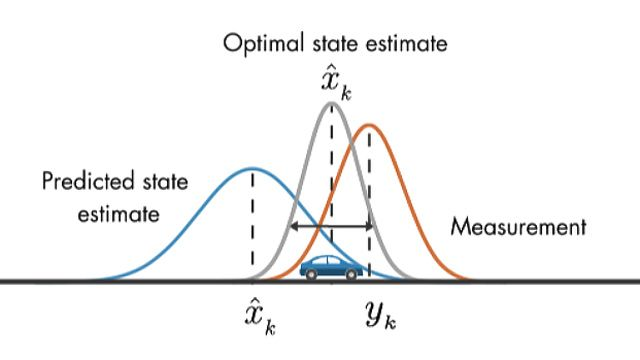
\includegraphics[width=1.0\linewidth]{images/kalman_2.jpg}
    \caption{Kalman filter prediction of the state using estimations. From: \cite{mathworks_kalman}.}
    \label{fig: Kalman filter prediction of the state using estimations.}
\end{figure}
\FloatBarrier\noindent

The Kalman filter follows a classical predict-update model, focusing on a single state variable: the vehicle’s velocity. The process and measurement uncertainty are encapsulated in the following variables:
\begin{itemize}
    \item Process variance Q: models the uncertainty in the vehicle’s motion (e.g., acceleration changes, jitter).
    \item Measurement variance R: represents the uncertainty in each self-speed estimation sample.
\end{itemize}

Where in real life the implementation can be represented as:
\begin{itemize}
    \item Estimated value: the current velocity estimate.
    \item Estimated error: the uncertainty (variance) of the current estimate.
\end{itemize}
At each new frame, a new self-speed estimation is used to update the Kalman filter which effects its output by a variable which is called Kalman Gain 'K':
\begin{equation}
K = \frac{\hat{P}}{\hat{P} + R}
\end{equation}
Where:
\begin{itemize}
    \item $\hat{P}$: predicted error variance
    \item $R$: measurement variance
\end{itemize}
This process allows the filter to balance trust between the incoming measurement and the current estimate. Over time, the filter becomes more confident, reducing the influence of noisy measurements.

Thus, the incorporation of the Kalman filter in this project provides smoother, more reliable self-speed estimation, which enhances the performance of the following dynamic filtering stage.

\begin{figure}[!htbp]
    \centering
    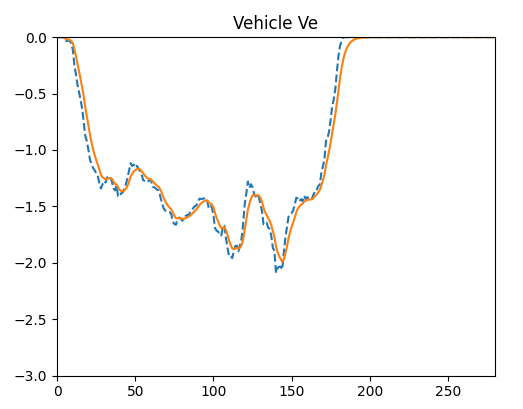
\includegraphics[width=1.0\linewidth]{images/kalman.png}
    \caption{Raw self-speed vs. self-speed after Kalman filter.}
    \label{fig: Test vehicle actual speed vs estimated speed.}
\end{figure}

\newpage
\subsection{Clustering}
Clustering is a key technique for grouping similar data points based on their spatial or statistical characteristics. 
In automotive sensing, clustering enables the detection and tracking of relevant objects such as vehicles, pedestrians, and obstacles by structuring raw radar detections into meaningful groups.

Among commonly used clustering algorithms, DBSCAN (Density-Based Spatial Clustering of Applications with Noise) stands out due to its robustness in handling irregular cluster shapes and its ability to automatically identify noise points without requiring a predefined number of clusters \cite{geeksforgeeks_dbscan}. 
This contrasts with centroid-based methods such as K-Means, which require specifying $K$ in advance and struggle with irregularly shaped clusters, and with hierarchical methods like agglomerative clustering, which can capture hierarchical structures but are computationally expensive and sensitive to noise.

\begin{table}[htbp]
\centering
\resizebox{\columnwidth}{!}{%
\begin{tabular}{|l|l|p{3.5cm}|p{3.5cm}|p{3.5cm}|}
\hline
\textbf{Algorithm} & \textbf{Type} & \textbf{Strengths} & \textbf{Weaknesses} & \textbf{Best Use Case} \\ \hline
DBSCAN & Density-Based & \begin{itemize}
    \item Detects clusters of varying shapes and sizes
    \item Identifies outliers (noise points)
\end{itemize} & \begin{itemize}
    \item Computationally expensive for large datasets
\end{itemize} & Radar object detection with dynamic object counts and noise filtering \\ \hline
K-Means & Centroid-Based & \begin{itemize}
    \item Fast and efficient for large datasets
\end{itemize} & \begin{itemize}
    \item Requires fixed number of clusters ($K$)
    \item Poor performance with irregular shapes
\end{itemize} & Structured radar data with known object counts \\ \hline
Agglomerative & Hierarchical & \begin{itemize}
    \item No prior knowledge of cluster number required
    \item Can detect hierarchical structures
\end{itemize} & \begin{itemize}
    \item Sensitive to noise
    \item High computational cost
\end{itemize} & Offline grouping of radar signatures \\ \hline
\end{tabular}% 
}
\caption{Comparison of clustering algorithms.}
\label{tab:clustering_algorithms}
\end{table}

DBSCAN defines a cluster based on two parameters: a neighborhood radius $\varepsilon$ and a minimum number of points $\text{MinPts}$.  
For a given point $p_i$ with coordinates $(x_i, y_i)$, its $\varepsilon$-neighborhood is defined as

\begin{equation}
    \mathcal{N}_{\varepsilon}(p_i) = \{ p_j \mid \lVert p_j - p_i \rVert_2 \leq \varepsilon \}.
\end{equation}

A point $p_i$ is called a \textit{core point} if
\begin{equation}
    |\mathcal{N}_{\varepsilon}(p_i)| \geq \text{MinPts}.
\end{equation}

Clusters are then formed by connecting density-reachable points, while points that do not belong to any cluster are classified as noise.  
This density-based formulation makes DBSCAN well-suited for radar data, where detections of the same object tend to be locally dense, while clutter appears as isolated points.

\subsubsection*{Two-Stage DBSCAN Rationale}
In practice, a single parameter set for $(\varepsilon, \text{MinPts})$ is insufficient because:
\begin{itemize}
    \item A large $\varepsilon$ merges nearby objects into one cluster.
    \item A small $\varepsilon$ causes fragmentation or discards weak reflections.
\end{itemize}

To address this, a two-stage DBSCAN process was implemented:

\paragraph{Stage 1: Permissive Filtering}
\begin{equation}
    \varepsilon_1 = \SI{2}{\meter}, \quad \text{MinPts}_1 = 2
\end{equation}
This stage acts as a noise filter by discarding points that cannot form even small local clusters.  
Outliers are eliminated early, reducing computational load for the next stage.

\paragraph{Stage 2: Fine Clustering}
\begin{equation}
    \varepsilon_2 = \SI{1}{\meter}, \quad \text{MinPts}_2 = 4
\end{equation}
This stage applies stricter parameters to avoid merging distinct objects into a single cluster.  
It ensures compact clusters that more accurately reflect real objects in the environment.

\begin{figure}[!htbp]
    \centering
    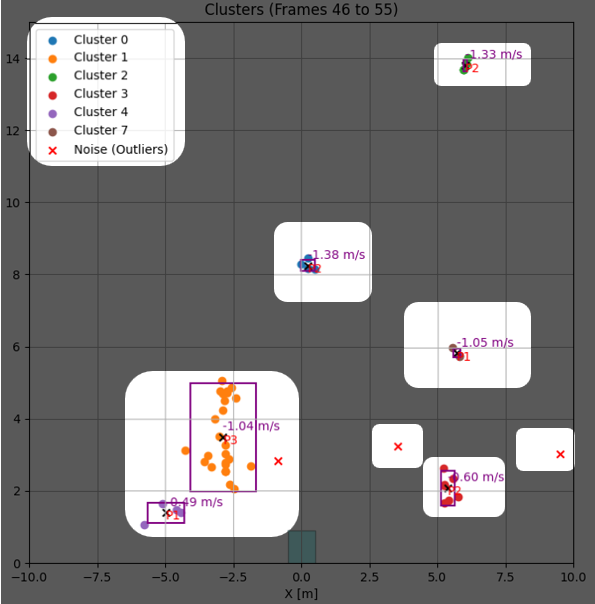
\includegraphics[width=1.0\linewidth]{images/clustering.png}
    \caption{Illustration of the first clustering stage: isolated outliers are discarded, and only candidate clusters remain.}
    \label{fig:first_clustering_stage}
\end{figure}

The resulting process can be expressed as a composition of the two operators:
\begin{equation}
    \mathcal{C}_{\text{final}} = \text{DBSCAN}(\varepsilon_2, \text{MinPts}_2, \; \text{DBSCAN}(\varepsilon_1, \text{MinPts}_1, \; P)),
\end{equation}
where $P$ denotes the raw radar point cloud and $\mathcal{C}_{\text{final}}$ the final set of clusters.  

This formulation highlights the dual role of DBSCAN: first as a noise filter, then as a clustering method.  
By structuring the problem in two passes, the algorithm maintains robustness to noise while achieving finer object separation in dense scenarios.

\subsection{Cluster Tracking}
\label{subsec:cluster_tracking}

Once clusters have been identified, it is necessary to track them over consecutive frames to ensure temporal consistency. 
A cluster tracker assigns each detected cluster a unique identifier (ID) and maintains a history of its trajectory over time. 
This enables the system to distinguish between persistent static objects and transient detections caused by noise or dynamic obstacles.

\subsubsection*{Hits and Misses}
Each tracked cluster is updated at every frame using two indices: 
\begin{itemize}
    \item \textbf{Hit Count ($h$):} The number of consecutive frames in which the cluster has been successfully matched to a detection.
    \item \textbf{Miss Count ($m$):} The number of consecutive frames in which the cluster has failed to find a corresponding detection.
\end{itemize}

A cluster is considered \textit{active} if $m \leq M_{\text{max}}$, where $M_{\text{max}}$ is the maximum allowed misses before deletion. 
This mechanism ensures that short occlusions or temporary sensor noise do not cause immediate loss of tracks.

\subsubsection*{Geometric Association}
Let $c_t = (x_t, y_t)$ denote the centroid of a cluster at frame $t$.  
For each existing track, association with a new detection is performed by minimizing the spatial distance:

\begin{equation}
    d(c_t, c_{t+1}) = \lVert c_t - c_{t+1} \rVert_2.
\end{equation}

If a fitted motion model is available, the distance is instead evaluated relative to the predicted cluster trajectory. 
In this project, a simple line-fitting approach was applied to the history of each cluster’s centroids:

\begin{equation}
    y = m x + b,
\end{equation}

where $(m,b)$ are obtained via least-squares regression over the last $N$ centroids.  
The orthogonal distance of a new detection $(x_0, y_0)$ to this fitted line is computed as:

\begin{equation}
    d_{\perp}(x_0, y_0) = \frac{|m x_0 - y_0 + b|}{\sqrt{m^2 + 1}}.
\end{equation}

The detection is associated with the track if $d_{\perp} \leq d_{\text{max}}$, where $d_{\text{max}}$ is a configurable threshold.

\subsubsection*{Track Management}
The complete tracking procedure consists of:
\begin{enumerate}
    \item \textbf{Initialization:} If no tracks exist, each cluster spawns a new track with a unique ID.
    \item \textbf{Association:} Existing tracks are matched to current detections using the minimum distance criterion.
    \item \textbf{Update:} Matched tracks increment their hit count ($h \leftarrow h+1$), reset their miss count, and append the centroid to their history.
    \item \textbf{New Track Creation:} Unmatched detections start new tracks with fresh IDs.
    \item \textbf{Deletion:} Tracks exceeding $M_{\text{max}}$ consecutive misses are deleted.
\end{enumerate}

This process ensures that each stationary object is consistently represented by the same track ID across frames, while spurious detections are naturally filtered out.

\begin{figure}[!htbp]
    \centering
    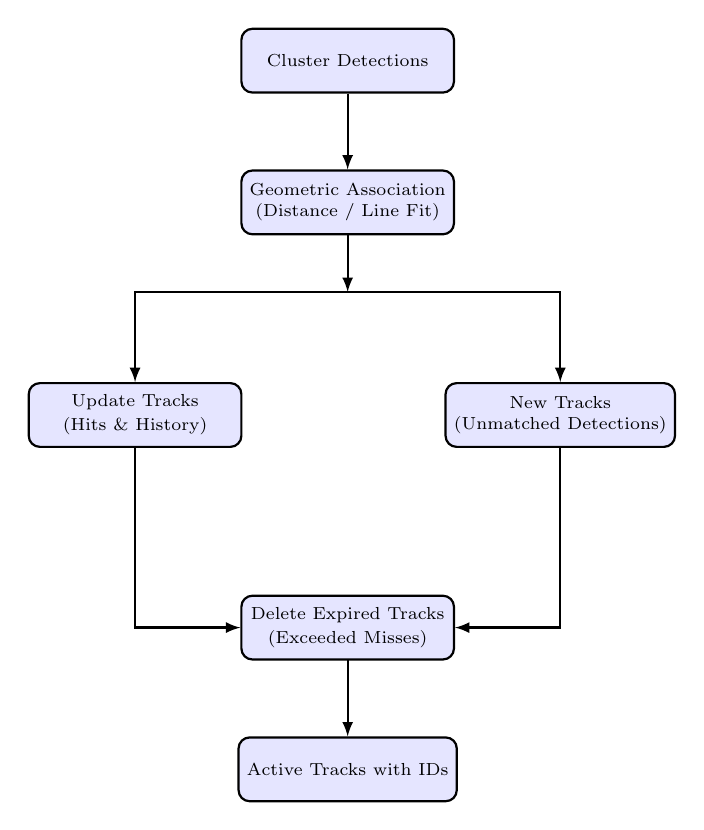
\begin{tikzpicture}[>=latex,thick,scale=0.9, every node/.style={scale=0.9}]
        % Styles
        \tikzstyle{block} = [rectangle, draw, fill=blue!10,
                             rounded corners, minimum height=0.9cm,
                             minimum width=3cm, align=center, font=\scriptsize]
        \tikzstyle{arrow} = [->, thick]

        % ==== Nodes (closer spacing, narrower width) ====
        \node[block] (input)        at (0,0)      {Cluster Detections};
        \node[block] (association)  at (0,-2)     {\shortstack{Geometric Association\\(Distance / Line Fit)}};
        \node[block] (update)       at (-3,-5)    {\shortstack{Update Tracks\\(Hits \& History)}};
        \node[block] (newtrack)     at (3,-5)     {\shortstack{New Tracks\\(Unmatched Detections)}};
        \node[block] (deletion)     at (0,-8)     {\shortstack{Delete Expired Tracks\\(Exceeded Misses)}};
        \node[block] (output)       at (0,-10)    {Active Tracks with IDs};

        % ==== Arrows ====
        \draw[arrow] (input) -- (association);

        % T-branch: down, then split left/right
        \draw[arrow] (association.south) -- ++(0,-0.8) coordinate (branch);
        \draw[arrow] (branch) -| (update.north);
        \draw[arrow] (branch) -| (newtrack.north);

        % Merge toward deletion
        \draw[arrow] (update.south) |- (deletion.west);
        \draw[arrow] (newtrack.south) |- (deletion.east);

        % Final output
        \draw[arrow] (deletion) -- (output);
    \end{tikzpicture}
    \caption{Cluster tracking block diagram. Each detection is associated with existing tracks or used to initialize new tracks. Tracks are deleted after exceeding miss thresholds.}
    \label{fig:cluster_tracking_block}
\end{figure}

To illustrate the method, Figure~\ref{fig:track_cluster_pointcloud} shows a clustered radar point cloud without temporal tracking.  
Figure~\ref{fig:track_cluster_tracked} shows the same scene after applying the tracker: each cluster is assigned an ID, along with Doppler, centroid coordinates, and hit count.  
The tracker maintains these IDs consistently across frames, enabling reliable identification of stationary obstacles.

\begin{figure}[!htbp]
    \centering
    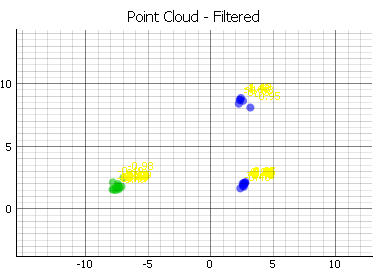
\includegraphics[width=0.48\linewidth]{images/TrackClusterPointCloud.png}
    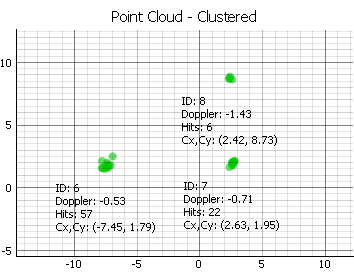
\includegraphics[width=0.48\linewidth]{images/TrackCluster.png}
    \caption{Illustration of the cluster tracking process. Left: clustered point cloud without tracking. Right: tracked clusters with assigned IDs, Doppler values, centroids, and hit counts.}
    \label{fig:track_cluster_pointcloud}
\end{figure}

\vspace{10\baselineskip}
\subsection{Iterative Closest Point (ICP)}
\label{subsec:icp}

The Iterative Closest Point (ICP) algorithm is a classical method for estimating rigid-body transformations between two point sets. 
In the context of radar odometry, ICP provides a way to align consecutive frames of radar point clouds in order to estimate ego-motion. 
The main goal is to determine the relative rotation $R \in SO(2)$ and translation $t \in \mathbb{R}^2$ that minimize the alignment error between a source point cloud $P = \{p_i\}_{i=1}^N$ and a target point cloud $Q = \{q_j\}_{j=1}^M$.

\subsubsection*{Mathematical Formulation}
The ICP algorithm can be separated into two main steps: correspondence search and transformation estimation.

\paragraph{Correspondence Search.}
For each point $p_i \in P$, the closest point in $Q$ is selected according to the Euclidean distance:
\begin{equation}
    q^*_i = \arg \min_{q_j \in Q} \lVert p_i - q_j \rVert_2.
\end{equation}
This step establishes a set of tentative correspondences $\{(p_i, q^*_i)\}$ between the two frames. 
Efficient implementations use spatial data structures such as KD-trees to accelerate nearest-neighbor searches.

\paragraph{Transformation Estimation.}
Once correspondences are found, the rigid-body transformation $(R,t)$ is estimated by minimizing the least-squares error:
\begin{equation}
    E(R,t) = \sum_{i=1}^{N} \lVert p_i - (R q^*_i + t) \rVert^2.
\end{equation}
The optimal solution can be obtained using singular value decomposition (SVD) of the cross-covariance matrix between the two point sets. 
In 2D, the rotation can be parameterized by an angle $\theta$, such that:
\begin{equation}
    R(\theta) = 
    \begin{bmatrix}
        \cos\theta & -\sin\theta \\
        \sin\theta & \cos\theta
    \end{bmatrix}.
\end{equation}

The transformation is then applied to $Q$, and the process is repeated iteratively until convergence, typically when changes fall below a threshold or a maximum number of iterations is reached.

\subsubsection*{Global ICP}
In the global variant, all available points of the radar point cloud are used to compute correspondences and estimate the motion. 
This maximizes the use of sensor information but can be sensitive to noise and dynamic objects, since outliers directly affect the transformation estimate.

\subsubsection*{Cluster-wise ICP}
To increase robustness, a cluster-wise approach was also investigated. 
Instead of using the entire point cloud, correspondences are restricted to clusters identified in the previous stage (see Section~\ref{subsec:cluster_tracking}). 
Among these clusters, priority is given to those with the highest \emph{hit count} and lowest \emph{miss count}, since they are more likely to represent stable, stationary objects. 
For each cluster $C_k$, an independent ICP alignment is performed:
\begin{equation}
    E_k(R,t) = \sum_{p_i \in P_k} \lVert p_i - (R q^*_i + t) \rVert^2,
\end{equation}
where $P_k$ and $Q_k$ denote corresponding cluster subsets across two consecutive frames.
The resulting transformations are then aggregated, typically via weighted averaging based on cluster stability, to obtain the final ego-motion estimate.

\subsubsection*{Practical Considerations}
Several practical aspects influence ICP performance:
\begin{itemize}
    \item \textbf{Initialization:} ICP assumes small inter-frame motion. Poor initialization may cause convergence to local minima.
    \item \textbf{Nearest-neighbor search:} KD-trees enable efficient correspondence search in $\mathcal{O}(N \log N)$ time.
    \item \textbf{Outlier rejection:} Correspondences with distances exceeding a threshold $d_{\max}$ are discarded to reduce the influence of spurious points.
    \item \textbf{Cluster selection:} Restricting ICP to stable clusters improves robustness against moving objects and noise.
\end{itemize}

\subsection{Iterative Closest Point (ICP) for Ego-Motion Estimation}
\label{subsec:icp}

The Iterative Closest Point (ICP) algorithm estimates the rigid-body transformation 
between two consecutive radar frames. Given two point sets
\[
P = \{p_i \in \mathbb{R}^2 \}_{i=1}^{N}, \quad
Q = \{q_j \in \mathbb{R}^2 \}_{j=1}^{M},
\]
the goal is to find a rotation $R \in SO(2)$ and translation $t \in \mathbb{R}^2$ that minimize the alignment error
\[
\min_{R,t} \sum_{i=1}^N \lVert R p_i + t - q_{\pi(i)} \rVert^2,
\]
where $\pi(i)$ denotes the index of the nearest neighbor of $p_i$ in $Q$.

\subsubsection*{Nearest Neighbor Matching}
To associate points between frames, a KD-tree was constructed over the set $Q$.  
For each point $p_i \in P$, its closest match $q_{\pi(i)}$ is obtained as:
\[
\pi(i) = \arg\min_j \lVert p_i - q_j \rVert_2.
\]

\subsubsection*{Per-Point Motion Estimates}
For each matched pair $(p_i, q_{\pi(i)})$, the incremental translation and orientation change are computed as
\[
t_i = p_i - q_{\pi(i)}, \qquad
\theta_i = \arctan2\!\left( (p_i - q_{\pi(i)})_y, (p_i - q_{\pi(i)})_x \right).
\]

\subsubsection*{Global Averaging}
The global motion is obtained by averaging over all matched pairs:
\[
\bar{t} = \frac{1}{N} \sum_{i=1}^N t_i, \qquad
\bar{\theta} = \frac{1}{N} \sum_{i=1}^N \theta_i.
\]

\subsubsection*{Homogeneous Transformation Matrices}
The estimated transformation from ICP is expressed in homogeneous coordinates as:
\[
T_{\text{ICP}} =
\begin{bmatrix}
\cos\bar{\theta} & -\sin\bar{\theta} & \bar{t}_x \\
\sin\bar{\theta} &  \cos\bar{\theta} & \bar{t}_y \\
0 & 0 & 1
\end{bmatrix}.
\]

For ego-motion estimation (inverse motion), the corresponding matrix is:
\[
T_{\text{ego}} =
\begin{bmatrix}
\cos\bar{\theta} & \sin\bar{\theta} & -(\bar{t}_x \cos\bar{\theta} + \bar{t}_y \sin\bar{\theta}) \\
-\sin\bar{\theta} & \cos\bar{\theta} & \;\;\bar{t}_x \sin\bar{\theta} - \bar{t}_y \cos\bar{\theta} \\
0 & 0 & 1
\end{bmatrix}.
\]

\subsubsection*{Cluster-wise ICP}
In addition to the global ICP (using all points), a cluster-wise ICP is applied.  
Each cluster $C_k$ maintains counters for \emph{hits} and \emph{misses}, ensuring stable targets are prioritized.  
For each cluster, the transformation $(t_k, \theta_k)$ is estimated using the above procedure.  
The global motion estimate is then computed as a weighted average:
\[
\bar{t} = \frac{\sum_k w_k t_k}{\sum_k w_k}, \qquad
\bar{\theta} = \frac{\sum_k w_k \theta_k}{\sum_k w_k},
\]
with weights
\[
w_k = \max\!\left(\min\!\left(\text{hits}_k^{\alpha}, \; \text{max\_hits}\right), 1\right),
\]
where $\alpha \in [1,2]$ controls the influence of stable clusters.

\subsubsection*{Python-style Conceptual Flow}
\begin{enumerate}
    \item Input two frames $P$ and $Q$.
    \item Use a KD-tree to find nearest neighbors between $P$ and $Q$.
    \item For each matched pair $(p_i,q_{\pi(i)})$, compute translation $(t_x,t_y)$ and rotation $\theta$.
    \item Average all translations and rotations to obtain $(\bar{t},\bar{\theta})$.
    \item Build the homogeneous transformation $T_{\text{ICP}}$.
    \item Derive the inverse ego-motion matrix $T_{\text{ego}}$.
    \item (\textbf{Cluster ICP}) Repeat steps 2–6 on each cluster and fuse results using hit-based weighting.
\end{enumerate}

\section{Summary and Outlook}

% Summary and leasons learned
In this project, an object detection system for a consumer-grade electric go-kart was implemented by using a mmWave radar sensor.
The system successfully meets its primary objectives by accurately detecting obstacles through a custom point-cloud analysis algorithm.
Although the current implementation is limited to stationary objects, it establishes a strong foundation for future development.
All necessary components, including a modular processing pipeline and a hardware interface for safely manipulating the go-kart's brake signal, were developed.
\par
The pipeline's modular architecture proved to support a dynamic developing process, which turned out to be necessary when working with point clouds from radar sensors and an electric go-kart that was not intended to be modified by the end-user.
It also enables further development by expanding, exchanging or modifying processing stages.
During the development, two stages turned out to be extraordinary helpful when it comes to mitigating the influences of the potentially heavily fluctuating point cloud data.
The frame aggregator in combination with running the radar sensor at a high frame rate successfully tackled the problem of data sparsity that sometimes occurred in the test scenario environment.
This was caused by the scenario's "clean" setup without a huge number of targets.
The two-stage clustering approach using the DBSCAN algorithm proved to be able to reliably filter out outliers caused by clutter or noise and was able to provide the brake controller with stable information on stationary objects.
\par
In addition to those two stages, the usage of multiple filtering stages of static and dynamic behavior proved to support the reliability of the whole system.
Static filtering stages early in the pipeline are able to filter out irrelevant points or those with a low level of confidence by using their spatial coordinates and $SNR$ information.
This reduces the required processing time of the later stages by condensing the mass of data to the relevant points.
The dynamic filtering stage allows a reliable differentiation between points that are caused by stationary and moving targets by leveraging the information of the radar-only self-speed estimation.
The approach of using a distance that is linear to the vehicle's velocity to decide whether an emergency braking event should be triggered, and outputting a binary signal, turned out to be sufficient, as the balance board's internal controller prevents the wheels from locking.
\par\bigskip
As with any project, there is always room for improvement, and this work is no exception.
Although the current implementation meets the initial goals and requirements, the algorithm can still be refined.
The project is currently implemented in a threaded solution using Python, which is a result of the dynamic development process where a lot of different techniques and approaches where implemented, tested and sometimes discarded.
Switching from C++, which was used initially used for development, to Python allowed for a quicker development with simpler possibilities of visualization, but also caused a noticeable lack of performance.
This lack of performance showed up in the last stages of development, during testing, and created a delay in the response when tested in an autonomous environment, meaning that when the implementation was not powered by a sufficient power supply, the implemented system showed certain delays in the response when an object was detected in the area for activation of the brake.
It is assumed that the delay originates from Python's heavyweight interpreter and should vanish after porting the system's implementation back to C++.
As for this reason, the decision of not fully merging the existing system into the test vehicle at this stage of the development was made, as it did not provided a fully safe environment for testing.
The validation was done with a LED to indicate the activation of the emergency brake.
An improvement or next step would be to migrate the system back to C++, where the threaded implementation would provide a better response time for each running task.
Further improvements can also be made by incorporating occupancy grids through a Bayesian filter to enhance object detection, allowing the system to go beyond stationary targets.
By improving the system's object detection capabilities to cover moving targets, it would also be possible to estimate their direction of movement, which could significantly improve the driving assistance algorithm and contribute to accident prevention through a more precise analysis.
\par\bigskip
The present status of this project is available in the following GitHub repository: \href{https://github.com/LF-RoGu/Radar-mmWave}{Radar-mmWave on GitHub}.
%\section{WIP - Storing TikZ graphics}

\begin{figure}[!htbp]
    \centering
    \resizebox{0.48\textwidth}{!}{
        \begin{tikzpicture}
            % Block styles
            \tikzstyle{block} = [rectangle, draw, text width=4.5em, text centered, minimum width=6em, minimum height=4em]
            \tikzstyle{block_dashed} = [rectangle, draw, text width=2em, text centered, minimum width=4em, minimum height=4em, dashed]
            % Input and output
            \node[block, right=of antenna, minimum width=4em, minimum height=4em] (frames) {Frames};
            \node[block, right=of frames] (frame_aggr) {Frame\\Aggregator};
            \node[block, right=of frame_aggr] (coord_filter) {Filter\\$x,y,z$\\$\phi,SNR$};
            \node[block, right=of coord_filter] (self_speed_estim) {Self-speed Estimator};
            \node[block, right=of self_speed_estim] (self_speed_kalman) {Kalman Filter};
            \node[block, below=of self_speed_estim] (ve_speed_calc) {Calculation\\of $v_{e}$};
            \node[block, right=of ve_speed_calc] (ve_filter) {Filter\\$v_{e}$ vs. self-speed};
            \node[block, right=of ve_filter] (clustering) {Clustering};
            % Connections
            \draw[->] (frames) -- (frame_aggr); % Connection from antenna to RF amplifier
            \draw[->] (frame_aggr) -- (coord_filter);
            \draw[->] (coord_filter) -- (self_speed_estim);
            \draw[->] (coord_filter.south) |- (ve_speed_calc.west);
            \draw[->] (self_speed_estim) -- (self_speed_kalman);
            \draw[->] (self_speed_kalman) -- (ve_filter);
            \draw[->] (ve_speed_calc) -- (ve_filter);
            \draw[->] (ve_filter) -- (clustering);
        \end{tikzpicture}
    }
    \caption{Block diagram of the pipeline}
    \label{fig:block_diag_pipeline}
\end{figure}

\begin{figure}[!htbp]
    \centering
    \resizebox{0.48\textwidth}{!}{
        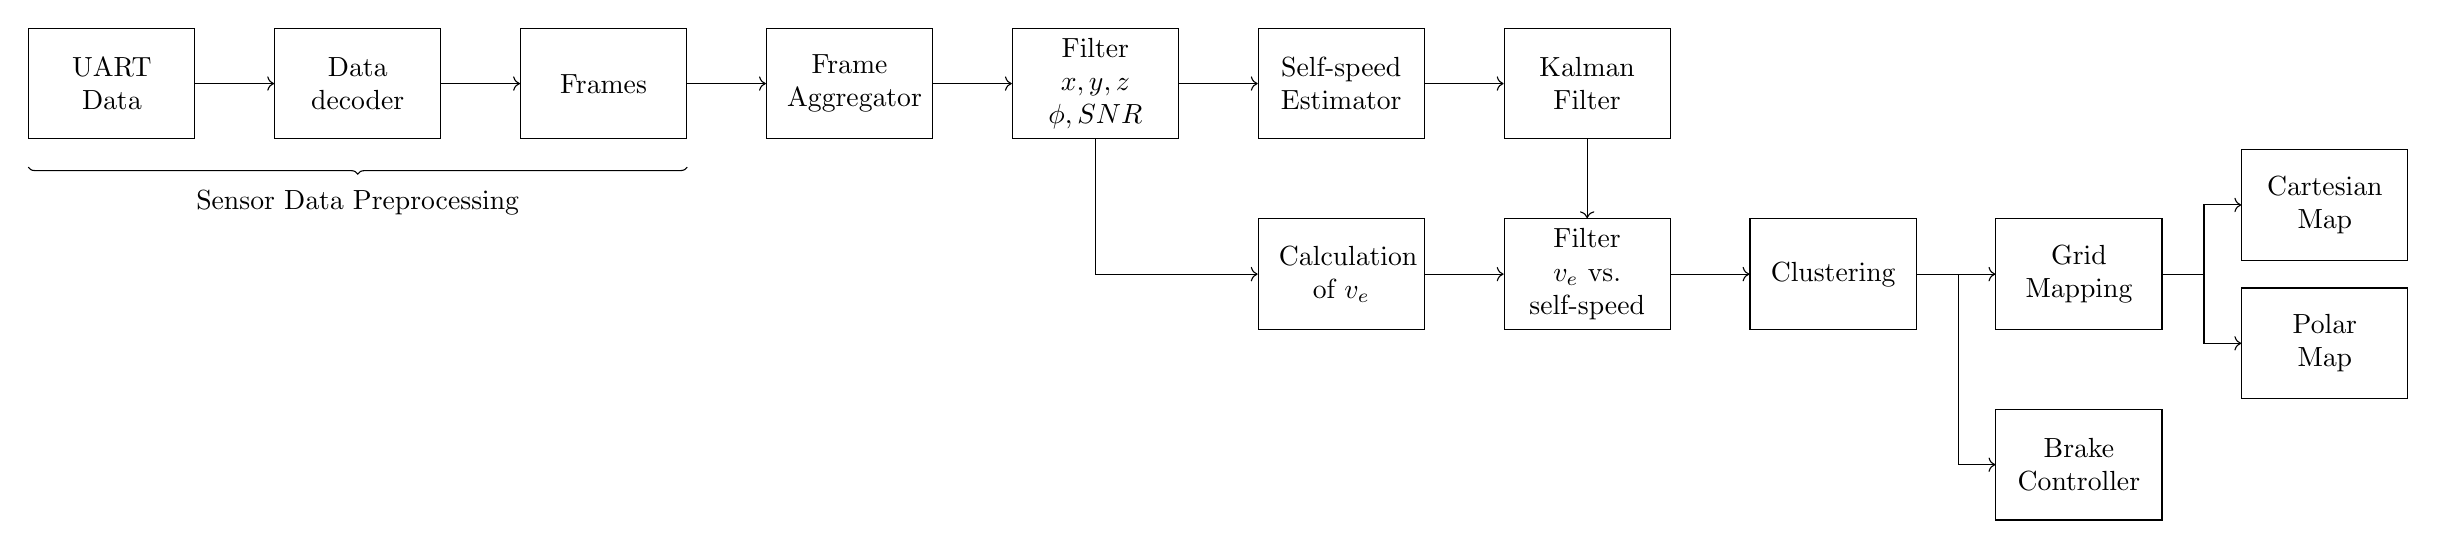
\begin{tikzpicture}
            % Block styles
            \tikzstyle{block} = [rectangle, draw, text width=4.5em, text centered, minimum width=6em, minimum height=4em]
            \tikzstyle{block_dashed} = [rectangle, draw, text width=2em, text centered, minimum width=4em, minimum height=4em, dashed]
            % Input and output
            \node[block] (uart) {UART\\Data};
            \node[block, right=of uart] (decoder) {Data decoder};
            \node[block, right=of decoder] (frames) {Frames};
            \node[block, right=of frames] (frame_aggr) {Frame\\Aggregator};
            \node[block, right=of frame_aggr] (coord_filter) {Filter\\$x,y,z$\\$\phi,SNR$};
            \node[block, right=of coord_filter] (self_speed_estim) {Self-speed Estimator};
            \node[block, right=of self_speed_estim] (self_speed_kalman) {Kalman Filter};
            \node[block, below=of self_speed_estim] (ve_speed_calc) {Calculation\\of $v_{e}$};
            \node[block, right=of ve_speed_calc] (ve_filter) {Filter\\$v_{e}$ vs. self-speed};
            \node[block, right=of ve_filter] (clustering) {Clustering};
            \node[block, right=of clustering] (grid_mapping) {Grid Mapping};
            \node[block, right=of grid_mapping.east, yshift=2.5em] (grid_cartesian) {Cartesian\\Map};
            \node[block, right=of grid_mapping.east, yshift=-2.5em] (grid_polar) {Polar\\Map};
            \node[block, below=of grid_mapping] (brake) {Brake\\Controller};
            % Connections
            \draw[->] (uart) -- (decoder);
            \draw[->] (decoder) -- (frames);
            \draw[->] (frames) -- (frame_aggr); % Connection from antenna to RF amplifier
            \draw[->] (frame_aggr) -- (coord_filter);
            \draw[->] (coord_filter) -- (self_speed_estim);
            \draw[->] (coord_filter.south) |- (ve_speed_calc.west);
            \draw[->] (self_speed_estim) -- (self_speed_kalman);
            \draw[->] (self_speed_kalman) -- (ve_filter);
            \draw[->] (ve_speed_calc) -- (ve_filter);
            \draw[->] (ve_filter) -- (clustering);

            \draw[-] (clustering.east) --++(1.5em, 0) coordinate (arrw_clustering);
            \draw[->] (arrw_clustering) -- (grid_mapping);
             \draw[->] (arrw_clustering) |- (brake);

            \draw[-] (grid_mapping.east) --++(1.5em, 0) coordinate (arrw_mapping_grids);
            \draw[->] (arrw_mapping_grids) |- (grid_cartesian.west);
            \draw[->] (arrw_mapping_grids) |- (grid_polar);

            \draw [decorate, decoration = {brace, mirror, raise=10pt}] (uart.south west) --  (frames.south east) node[pos=0.5,below=15pt,black]{Sensor Data Preprocessing};
        \end{tikzpicture}
    }
    \caption{Block diagram of the pipeline}
    \label{fig:block_diag_pipeline}
\end{figure}


\begin{figure}[!htbp]
    \centering
    \resizebox{0.48\textwidth}{!}{
        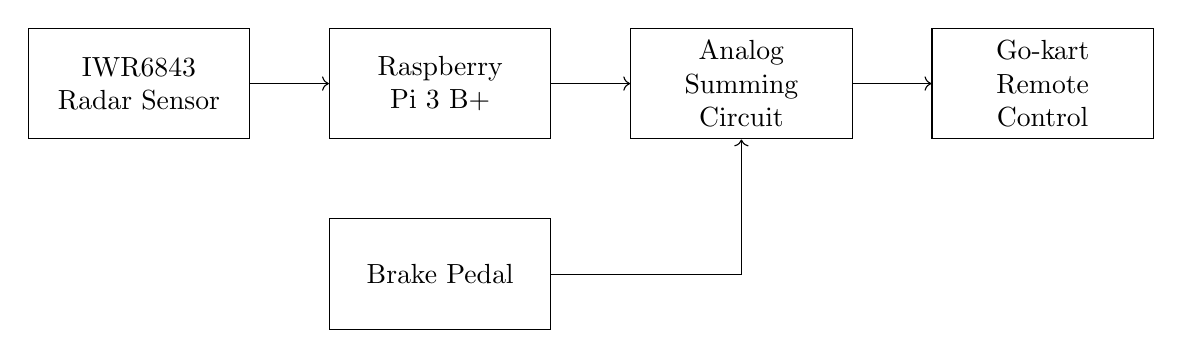
\begin{tikzpicture}
            % Block styles
            \tikzstyle{block} = [rectangle, draw, text width=6.5em, text centered, minimum width=8em, minimum height=4em]
            \tikzstyle{block_dashed} = [rectangle, draw, text width=2em, text centered, minimum width=4em, minimum height=4em, dashed]
            % Input and output
            \node[block] (radar) {IWR6843\\Radar Sensor};
            \node[block, right=of radar] (rpi) {Raspberry\\Pi 3 B+};
            \node[block, right=of rpi] (analog_summ) {Analog Summing\\Circuit};
            \node[block, below=of rpi] (brake_pedal) {Brake Pedal};
            \node[block, right=of analog_summ] (remote) {Go-kart\\Remote Control};
            % Connections
            \draw[->] (radar) -- (rpi);
            \draw[->] (rpi) -- (analog_summ);
            \draw[->] (brake_pedal) -| (analog_summ);
            \draw[->] (analog_summ) -- (remote);
        \end{tikzpicture}
    }
    \caption{Block diagram of the pipeline}
    \label{fig:block_diag_pipeline}
\end{figure}
\newpage

\begin{thebibliography}{00}

\bibitem{ninebot_product_page} Segway Inc., ``Ninebot Go-kart PRO product page'', 2025, Webpage. [Online]. Available: \url{https://de-de.segway.com/products/ninebot-gokart-pro}

\bibitem{iwr_awr_diff} Texas Instruments, ``IWR1642: difference between AWR and IWR parts'', 2025, Webpage. [Online]. Available: \url{https://e2e.ti.com/support/sensors-group/sensors/f/sensors-forum/742730/iwr1642-difference-between-awr-and-iwr-parts}

\bibitem{dev_board_page} Texas Instruments, ``IWR6843AOPEVM product page'', 2025, Webpage. [Online]. Available: \url{https://www.ti.com/tool/IWR6843AOPEVM}

\bibitem{mmwave_demo_doc} Texas Instruments, ``User's Guide mmWave Demo Visualizer,'' 2020, Online Document. [Online]. Available: \url{https://www.ti.com/lit/ug/swru529c/swru529c.pdf?ts=1742817596204}.

\bibitem{understanding_uart} Texas Instruments, ``Understanding UART Data Output Format'', 2025, Webpage. [Online]. Available: \url{https://dev.ti.com/tirex/content/radar_toolbox_2_20_00_05/docs/software_guides/Understanding_UART_Data_Output_Format.html}

\bibitem{mmwave_demo_output} Texas Instruments, ``mmWave Sensing Estimator'', 2025, Webpage. [Online]. Available: \url{https://dev.ti.com/gallery/view/mmwave/mmWaveSensingEstimator/ver/2.5.1/}


\bibitem{ninebot_protocol_github} ub4raf, ``Ninebot-PROTOCOL'', 2025, GitHub Repository. [Online]. Available: \url{https://github.com/ub4raf/Ninebot-PROTOCOL}

\bibitem{ninebot_protocol_scooterhacking} -, ``Ninebot ES Communicaton Protocol'', 2019, Webpage. [Online]. Available: \url{https://cloud.scooterhacking.org/release/nbdoc.pdf}

\bibitem{numpy_polyfit} -, ``numpy.polyfit documentation'', 2025, Webpage. [Online]. Available: \url{https://numpy.org/doc/stable/reference/generated/numpy.polyfit.html}

\bibitem{OccupancyGrid_Mapping_Automotive} Ç. Önen, A. Pandharipande, G. Joseph, and N. J. Myers, ``Occupancy Grid Mapping for Automotive Driving Exploiting Clustered Sparsity,'' \textit{IEEE Sensors Journal}, vol. 24, no. 7, pp. 9240-9250, 2024. [Online]. Available: \url{https://doi.org/10.1109/JSEN.2023.3342463}.

\bibitem{Odometry_radar_only}
D. Casado Herraez, M. Zeller, L. Chang, I. Vizzo, M. Heidingsfeld, and C. Stachniss, 
``Radar-Only Odometry and Mapping for Autonomous Vehicles,'' 
\textit{arXiv preprint}, 2023. [Online]. Available: \url{https://arxiv.org/abs/2305.12409}

\bibitem{EgoMotion_DopplerRadar}
S. R. Bhatt, B. S. Nadiger, R. Parthasarathy, and H. M. Shetty, 
``Instantaneous Ego-motion Estimation Using Doppler Radar,'' 
\textit{IEEE Sensors Letters}, vol. 7, no. 5, pp. 1–4, 2023. [Online]. Available: \url{https://doi.org/10.1109/LSENS.2023.3244030}

\bibitem{Multimodal_Offroad}
C. E. Beal, T. Williams, J. Pauli, M. Mukadam, and B. Boots, 
``Robust Off-Road Autonomy Using Multimodal Sensor Fusion,'' 
in \textit{Proc. of the Conference on Robot Learning (CoRL)}, 2023. [Online]. Available: \url{https://openreview.net/forum?id=kmiZqSgoAt}

\bibitem{HighSpeed_Estimation}
B. Sundaralingam, C. E. Beal, and B. Boots, 
``Robust High-Speed State Estimation for Off-Road Autonomous Vehicles,'' 
in \textit{Proc. of Robotics: Science and Systems (RSS)}, 2023. [Online]. Available: \url{https://openreview.net/forum?id=3JpFLY3ihix}


\bibitem{geeksforgeeks_dbscan}
GeeksforGeeks, 
\emph{DBSCAN Clustering in ML | Density Based Clustering}, 
2023. [Online]. Available: \url{https://www.geeksforgeeks.org/dbscan-clustering-in-ml-density-based-clustering/}. [Accessed: 19-Mar-2025].

\bibitem{mathworks_kalman}
MathWorks,
\textit{Understanding Kalman Filters, Part 3: Optimal State Estimator},
2017. Available at: \url{https://la.mathworks.com/videos/understanding-kalman-filters-part-3-optimal-state-estimator--1490710645421.html} (Accessed: March 23, 2025).

\bibitem{ti_radar_toolbox}
Texas Instruments, 
\textit{Radar Toolbox – mmWave Sensor Configuration and Demos}, 
2024. Available at: \url{https://dev.ti.com/tirex/explore/node?node=A__ADnbI7zK9bSRgZqeAxprvQ__radar_toolbox__1AslXXD__2.20.00.05} (Accessed: March 23, 2025).




\end{thebibliography}


\end{document}

\begin{comment}
    [25/09/2025]
    The new structure shall be
    - Abstract.
    - Introduction.
    - Objective.
        - Why are we doing this.
        - What are the benefits.
    - System Hardware.
        - Talk about the sensors, briefly.
        - 3D printed parts.
            - Showcase of models.
            - Showcase of implementation.
        - mmWave.
            - Calibration.
            - Chirp configuration.
        - IMU.
            - Calibration.
        - Webcam.
    - Pipeline.
        - Transformations.
        - Frame Aggregator.
        - Filtering.
        - RANSAC.
        ...
        - ICP.
    - Solution discussion.
    - Bibliography.
\end{comment}